\documentclass[IEEM]{HKA} % The options IEEM, MMT, and EIT are available
% Wird verwendet, um die Seitenränder schmäler zu machen. Es kann passieren, dass 
% jede zweite Seite nach rechts versetzt ist. Das soll beim Druck dabei helfen, dass 
% auch auf der rechten Seite noch alles gut zu lesen ist.
%\KOMAoptions{DIV=13}

%%%%%%%%%%%%%%%%%%%%%%%%%%%%%%%%%%%%%%%%%%%%%%%%%%%%%%%%%%%%%%%%%%%%%%%%%%%%%%%%%%%%%%%%%%%%%%%%%%%%%%
%	LANGUAGE
%%%%%%%%%%%%%%%%%%%%%%%%%%%%%%%%%%%%%%%%%%%%%%%%%%%%%%%%%%%%%%%%%%%%%%%%%%%%%%%%%%%%%%%%%%%%%%%%%%%%%%
\setdefaultlanguage{german} % english or german 



%%%%%%%%%%%%%%%%%%%%%%%%%%%%%%%%%%%%%%%%%%%%%%%%%%%%%%%%%%%%%%%%%%%%%%%%%%%%%%%%%%%%%%%%%%%%%%%%%%%%%%
%	PACAKGES
%%%%%%%%%%%%%%%%%%%%%%%%%%%%%%%%%%%%%%%%%%%%%%%%%%%%%%%%%%%%%%%%%%%%%%%%%%%%%%%%%%%%%%%%%%%%%%%%%%%%%%
% This package is only used in the demo and should be removed for the actual thesis.
\usepackage[backgroundcolor=white,linecolor=red,bordercolor=red,textsize=footnotesize]{todonotes}
% Wird benötigt, um Grafiken einzufügen
\usepackage{graphicx}
\usepackage{tabularx}
% Wird für Tabellen benötigt
\usepackage{booktabs} 
\usepackage[nohyperlinks, printonlyused]{acronym}
% Wird benötigt, um selbst Grafiken zeichnen zu können
\usepackage{tikz}
% Wird benötigt, um bestimmte Symbole in Abbildungen zu zeichnen
\usepackage{amsmath}
\usepackage{amssymb}
% Wird benötigt, um Wikel zeichnen zu können
\usetikzlibrary{angles, quotes}
% Wird zur besseren Positionierung von Grafiken oder Tabellen gebraucht
\usepackage{float}
\usepackage[utf8]{inputenc}
% Dieses Paket wird benötigt, um automatisch ein Abkürzungsverzeichnis zu generieren
\usepackage{glossaries}





%%%%%%%%%%%%%%%%%%%%%%%%%%%%%%%%%%%%%%%%%%%%%%%%%%%%%%%%%%%%%%%%%%%%%%%%%%%%%%%%%%%%%%%%%%%%%%%%%%%%%%
%	COMMANDS
%%%%%%%%%%%%%%%%%%%%%%%%%%%%%%%%%%%%%%%%%%%%%%%%%%%%%%%%%%%%%%%%%%%%%%%%%%%%%%%%%%%%%%%%%%%%%%%%%%%%%%
%\newcommand{cmd}{def} Define new commands if necessary
\graphicspath{ {./Bilder/} }



%%%%% Glossar 
\makeglossaries



\newglossaryentry{latex}
{
	name=latex,
	description={Is a markup language specially suited for scientific documents}
}

\newglossaryentry{Spawnpunkt}
{
	name=Spawnpunkt,
	description={Bezeichnet eine 2D oder 3D Koordinate in einer Simulationsumgebung oder in einem Videospiel, an welchem virtuelle Objekte instanziiert werden}
}

%%%%%% Abkürzungsverzeichnis 

\newacronym{api}{API}{Application Programming Interface}

\newacronym{rgb}{RGB}{Rot, Grün, Blau (Farbraum)}

\newacronym{id}{ID}{Identifikationsnummer}

\newacronym{sdk}{SDK}{Software Development Kit}



%%%%%%%%%%%%%%%%%%%%%%%%%%%%%%%%%%%%%%%%%%%%%%%%%%%%%%%%%%%%%%%%%%%%%%%%%%%%%%%%%%%%%%%%%%%%%%%%%%%%%%
%	META DATA
%%%%%%%%%%%%%%%%%%%%%%%%%%%%%%%%%%%%%%%%%%%%%%%%%%%%%%%%%%%%%%%%%%%%%%%%%%%%%%%%%%%%%%%%%%%%%%%%%%%%%%
% Comment out or delete what you don't need

% THESIS TYPE: One of the following types must be chosen
% \dissertation			- Dissertation
% \masterthesis			- Master Thesis
% \bachelorthesis		- Bachelor Thesis
% \projectbachelor		- Development Project (Bachelor)
% \projectmaster		- Development Project (Master)
% \firstprojectmaster	- Development and Research Project 1 (Master)
% \secondprojectmaster	- Development and Research Project 2 (Master)
\thesistype{\projectmaster} 


% NON-DISCLOSURE AGREEMENT. This only needs to be specified in case your work includes confidential information or data, for example, when your work is done in cooperation with an industry company. Otherwise, this command can be deleted or commented out. In case the non-disclosure agreement is necessary, a date and the name of the organisation needs to be provided. The date specifies the earliest point in time at which your work can be viewed by HKA memebers other than your supervisors and reviewers.
%\nonDisclosure{31.03.2028}{Example GmbH}


% ACADEMIC TITLE: Only necessary for dissertations, bachelor theses, and master theses.
\academicdegreeshort{M. Sc.}
\academicdegreefull{Master of Science}


% AUTHORS: 1 - 6 authors can be specified. Dissertations, bachelor, and master theses have one author
\place{Karlsruhe} % Birthplace of the author, only necessary for dissertations, bachelor theses, and master theses
\authors
{Lenard Haas} % Author 1
{Jonas Verleger} % Author 2
{} % ...
{}
{}
{}

\studentnumbers
{90272} % Student number author 1
{90922}  % Student number author 2
{} % ...
{}
{}
{}



% TITLE
\title{Implementierung eines Eye-Tracking Systems in den Fahrsimulator der Hochschule Karlsruhe}

% TIME FRAME
\timeframe{01.11.2025 - 01.06.2025} % Delete for dissertations
\submissiondate{Mai 2025}

% EXAMINERS: The dean is only necessary for student projects (maybe also for dissertations). The third examiner is usually necessary for theses in industry or for dissertations with an external reviewer.  
%\dean{Prof. Dr.-Ing. Robert Weiß} 

\firstexaminer
{Patrick Rebling M.Sc.}
{Institute of Energy Efficient Mobility}
{Karlsruhe University of Applied Sciences}

\secondexaminer
{Prof. Dr.-Ing. Philipp Nenninger}
{Institute of Energy Efficient Mobility}
{Karlsruhe University of Applied Sciences}


%%%%%%%%%%%%%%%%%%%%%%%%%%%%%%%%%%%%%%%%%%%%%%%%%%%%%%%%%%%%%%%%%%%%%%%%%%%%%%%%%%%%%%%%%%%%%%%%%%%%%%
%	BIBLIOGRAPHY
%%%%%%%%%%%%%%%%%%%%%%%%%%%%%%%%%%%%%%%%%%%%%%%%%%%%%%%%%%%%%%%%%%%%%%%%%%%%%%%%%%%%%%%%%%%%%%%%%%%%%%
% Loads bibliography for citations.
\preto\fullcite{\AtNextCite{\defcounter{maxnames}{99}}}


\addbibresource{literatur.bib}
% Sorgt dafür, dass die Abbildungsnummierung nicht die Kapitelnummerierung vor dem Komma stehen hat.
\counterwithout{equation}{chapter}
\counterwithout{figure}{chapter}

\setcounter{biburlnumpenalty}{10000} % break on URL numbers
\setcounter{biburllcpenalty}{10000} % break on URL lower case letters
\setcounter{biburlucpenalty}{10000} % break on URL UPPER CASE letters


%%%%%%%%%%%%%%%%%%%%%%%%%%%%%%%%%%%%%%%%%%%%%%%%%%%%%%%%%%%%%%%%%%%%%%%%%%%%%%%%%%%%%%%%%%%%%%%%%%%%%%
%	DOCUMENT
%%%%%%%%%%%%%%%%%%%%%%%%%%%%%%%%%%%%%%%%%%%%%%%%%%%%%%%%%%%%%%%%%%%%%%%%%%%%%%%%%%%%%%%%%%%%%%%%%%%%%%
\begin{document}
	
	%%%%%%%%%%%%%%%%%%%%%%%%%%%%%%%%%%%%
	%	FRONT MATTER
	%%%%%%%%%%%%%%%%%%%%%%%%%%%%%%%%%%%%
	% Comment out or delete inputs you don't need
	\frontmatter
	\maketitle
	%\acknowledge{%%%%%%%%%%%%%%%%%%%%%%%%%%%%%%%%%%%%%%%%%%%%%%%%%%%%%%%%%%%%%%%%%%%%%%%%%%%%%%%%%%%%%%%%%%%%%%%%%%%%%%
%	COMMENTS
%%%%%%%%%%%%%%%%%%%%%%%%%%%%%%%%%%%%%%%%%%%%%%%%%%%%%%%%%%%%%%%%%%%%%%%%%%%%%%%%%%%%%%%%%%%%%%%%%%%%%%
% Headline is created automatically

\textit{Example: I would like to take this opportunity to thank all those who accompanied and supported me in the preparation of this Master's thesis. I would like to thank Prof. ...} \newline


This section is used to thank people who have supported the author during the work. These may be supervising professors or doctoral students. In the case of work that took place in industry, the company or the supervisors can also be thanked. Furthermore, family and friends can be thanked. 

The acknowledgements are optional. For project work, an acknowledgement is rather unusual. For theses and dissertations in particular, it makes sense to thank the supervisors etc. involved.

}
	\abstract{%%%%%%%%%%%%%%%%%%%%%%%%%%%%%%%%%%%%%%%%%%%%%%%%%%%%%%%%%%%%%%%%%%%%%%%%%%%%%%%%%%%%%%%%%%%%%%%%%%%%%%
%	COMMENTS
%%%%%%%%%%%%%%%%%%%%%%%%%%%%%%%%%%%%%%%%%%%%%%%%%%%%%%%%%%%%%%%%%%%%%%%%%%%%%%%%%%%%%%%%%%%%%%%%%%%%%%
% Headline is created automatically

As part of this project, an eye tracker was implemented in a driving simulator at Karlsruhe University of Applied Sciences using inexpensive, commercially available hardware. The aim was to record the gaze position of test subjects in various traffic scenarios in order to analyse their perception and decision-making processes in road traffic more systematically. The aim of the project was not to develop a completely new tracking system from scratch. Instead, existing eye tracking systems were to be evaluated for their applicability in the university's driving simulator and implemented. The main part of the project consisted of finding a suitable eye tracking system, implementing it in the CARLA environment and finding solutions to any technical problems that might arise. 

After a market analysis, the Beam Eye Tracker from Eyeware Tech was selected due to its user-friendly API, low purchase price, low hardware requirements and accuracy that met the requirements of the application. The implementation was carried out using Python with the Beam SDK. The tracking data was linked to CARLA, in particular to the data from the Instance Segmentation Sensor, in order to infer the objects viewed in the simulation from the gaze position estimated by the eye tracker. This allows the eye tracker not only to output the test person's gaze position in x and y coordinates relative to the screen, but also to recognise which object the test person is looking at within the CARLA simulation environment at any given time. The interface between the eye tracker data and the CARLA Instance Segmentation Sensor data was tested in a specially created test environment in CARLA. 

A key technical problem was the curved projection screen of the driving simulator, which led to distortions in the recorded gaze data. To compensate for this, a software-based correction was implemented that uses mathematical functions to minimise the error caused by the curved screen. The accuracy of the implemented tracking system is sufficient to be able to determine which object the test person is looking at at any given time for larger objects in the CARLA simulation world. These are good results, especially considering the low financial outlay compared to eye tracking systems that cost several hundred euros. It was possible to implement the eye tracking system free of charge. The only costs incurred were those of the webcam used. Implementation in the driving simulator and in the CARLA environment was completed in full.

The work proves that even with inexpensive hardware and software, it is possible to functionally integrate eye tracking systems into driving simulators with large, curved screens, thus laying the foundation for future experiments in driving behaviour analysis. The work also identifies potential approaches for further improving tracking accuracy in the future. }
	\zusammenfassung{%%%%%%%%%%%%%%%%%%%%%%%%%%%%%%%%%%%%%%%%%%%%%%%%%%%%%%%%%%%%%%%%%%%%%%%%%%%%%%%%%%%%%%%%%%%%%%%%%%%%%%
%	COMMENTS
%%%%%%%%%%%%%%%%%%%%%%%%%%%%%%%%%%%%%%%%%%%%%%%%%%%%%%%%%%%%%%%%%%%%%%%%%%%%%%%%%%%%%%%%%%%%%%%%%%%%%%
% Headline is created automatically

This is a translation of the abstract into another language. In case your work is written in German, this page is usually in English and vice versa.
}
%	\publications{%%%%%%%%%%%%%%%%%%%%%%%%%%%%%%%%%%%%%%%%%%%%%%%%%%%%%%%%%%%%%%%%%%%%%%%%%%%%%%%%%%%%%%%%%%%%%%%%%%%%%%
%	COMMENTS
%%%%%%%%%%%%%%%%%%%%%%%%%%%%%%%%%%%%%%%%%%%%%%%%%%%%%%%%%%%%%%%%%%%%%%%%%%%%%%%%%%%%%%%%%%%%%%%%%%%%%%
% Headline is created automatically

This page is only relevant for dissertations! Here, you can list the primary publications \textbf{in which you are an author or co-author} and that are a part of your work or contribute to it. For example:

\begin{itemize}
	\item \fullcite{Rebling.2020}
	\item \fullcite{Kargl.2023}
	\item \fullcite{SommerAad.2019}
\end{itemize}

}
%	\furtherpublications{%%%%%%%%%%%%%%%%%%%%%%%%%%%%%%%%%%%%%%%%%%%%%%%%%%%%%%%%%%%%%%%%%%%%%%%%%%%%%%%%%%%%%%%%%%%%%%%%%%%%%%
%	COMMENTS
%%%%%%%%%%%%%%%%%%%%%%%%%%%%%%%%%%%%%%%%%%%%%%%%%%%%%%%%%%%%%%%%%%%%%%%%%%%%%%%%%%%%%%%%%%%%%%%%%%%%%%
% Headline is created automatically


Here, you can additional publications \textbf{in which you are an author or co-author}, but are not primarily relevant for your dissertation.}
	\tableofcontents
	\addcontentsline{toc}{chapter}{\contentsname}
	
	
	%%%%%%%%%%%%%%%%%%%%%%%%%%%%%%%%%%%%
	%	MAIN MATTER
	%%%%%%%%%%%%%%%%%%%%%%%%%%%%%%%%%%%%
	% Comment out or delete inputs you don't need. Add additional chapters if necessary
	\mainmatter
	\chapter{Einführung}
\label{sec:einführung}

Das menschliche Fahrverhalten ist bedingt durch die Vielzahl der möglichen Situationen im Straßenverkehr vielseitig. Um das Verhalten in verschiedenen Situationen zu untersuchen, müssen entweder Daten aus dem realen Verkehr ausgewertet werden oder bestimmte Situationen in einer kontrollierten Testumgebung nachgestellt werden. In einer realen Testumgebung ist es allerdings schwer, bestimmte Situationen gezielt nachzustellen. Die Umgebungsbedingungen des realen Verkehrs mit unterschiedlichen Fahrumgebungen wie Landstraßen, Autobahnen, Städten oder verschiedene Verkehrsteilnehmern wie Autofahrern, Straßenbahnen, Radfahrern und Fußgängern sind komplex. Ein anderer Ansatz ist es, die Umgebung zu simulieren. Auch für die Nachbildung von gefährlichen Situationen im Straßenverkehr weist eine Simulation aus finanzieller und praktischer Sicht Vorteile auf. Verschiedene Verkehrssituationen können mit kleineren finanziellen Aufwänden wiederholbar und zeitlich flexibel durchgeführt werden. Das Automotive Mobility Lab des Institus für energieeffiziente Mobilität ({\acs{IEEM}}) entwickelt aus diesem Grund ein Simulationsframework, welches mit unterschiedlichen Fortbewegungsmethoden (Auto, Fahrrad, Gehen) und in unterschiedlicher Realitätsnähe genutzt werden kann. Dadurch sind \Gls{Human-in-the-Loop}-Fahrversuche möglich, bei denen Fahrversuche mit einer realen Testperson in einer simulierten Umgebung durchgeführt werden können.  

Als Softwarebasis dient das Open-Source-Projekt \Gls{CARLA}. Dieses ermöglicht es, verschiedene Verkehrsszenarien nachzustellen. Die Analyse des menschlichen Verhaltens im Straßenverkehr kann somit ohne Gefahren und in vielfältigen simulierten Szenarien erfolgen. Die \Gls{Server-Client Struktur} von CARLA lässt ebenso mehrere Probanden in demselben Verkehrsszenario zu. So können menschliche Interaktionen realitätsnah nachgebildet werden.

Um die Ursachen bestimmter Entscheidungen im Straßenverkehr zu ergründen, soll in dem Fahrsimulator ein Eye Tracking System integriert werden. Durch die Auswertung der Blickposition des Fahrers sollen Informationen zum Wahrnehmungs- und Entscheidungsprozess des Fahrers in gewissen Situationen gewonnen werden. Hierdurch soll deutlich werden, was die Probanden während der Testfahrt sehen, worauf diese sich konzentrieren und welche Handlungsoptionen sie in Gefahrensituationen abwägen.

\newpage

\section{Zielsetzung}

Im Rahmen dieser Projektarbeit soll ein kamera basierter Eye Tracker in den Fahrsimulator der Hochschule bzw. in die CARLA Simulationsumgebung integriert werden.

Dazu sollen verschiedene verfügbare Eye Tracker auf die Anwendbarkeit und Integrierbarkeit in CARLA bewertet werden. Zur Erprobung des Eye Trackers soll ein Testszenario in CARLA erstellt werden. Weitere Vorgaben sind die Projektion des Blickpunktes auf die Leinwand und eine Ausgabe der aufgezeichneten Daten. Außerdem sollen die Daten innerhalb der Simulationsumgebung mit den Daten des Eye Trackers vereint werden. Dafür soll vor allem der \Gls{Instance Segmentation} Sensor innerhalb von CARLA zum Einsatz kommen. Dieser wird in einem späteren Abschnitt genauer erklärt. Ziel wird es sein, die Daten des Eye Trackers mit den Daten dieses Sensors zu vereinen, um Aussagen über die von der Testperson angeschauten Objekte in der Simulation zu erhalten.  


\section{Lösungsansatz}

Zur Zielerreichung müssen zuerst die Grundlagen von Eye Tracker Systemen und der CARLA-Simulationsumgebung erarbeitet werden. Für die Integration in das Gesamtsystem soll ein objektorientierter Python Code entwickelt werden. Damit die Ziele erreicht werden können, ist vor allem eine intensive Auseinandersetzung mit den Application Programming Interfaces ({\acs{API}})s der verschiedenen beteiligten Systemen notwendig. Eine Eigenentwicklung eines Eye Tracking Systems ist technisch und mathematisch anspruchsvoll und würde den zeitlichen Rahmen einer Projektarbeit übersteigen. Aus diesem Grund muss ein bereits vorhandenes System gefunden werden, welches kostengünstig ist und welches mindestens eine {\acs{API}} bietet, mit welcher die ausgegebenen Daten weiterverarbeitet werden können. Außerdem muss sichergestellt werden, dass die Krümmung der Leinwand bei der Verwendung des Eye Tracking Systems nicht zu Ungenauigkeiten führt. Entweder wird ein Eye Tracking System eingesetzt, welches gekrümmte Leinwände nativ unterstützt oder es muss eine selbst entwickelte Lösung erarbeitet werden. 







	\chapter{Eye Tracker}
\label{sec:eye tracker}

\section{Grundlegende Hardwarevoraussetzungen}

<<<<<<< HEAD
In diesem Kapitel wird ein grundlegender Einblick in die Hardwarevoraussetzungen für ein Eye Tracking System bereitgestellt. Daraufhin wird eine Marktanalyse durchgeführt, um verfügbare Eye Tracker auf deren Anwendbarkeit, Integration in CARLA und Kosten zu untersuchen.

Eye Tracking Systeme bestimmen die Mitte der Pupille, leiten die Rotation des Augapfels ab und bestimmen dann mithilfe von mathematischen Algorithmen die Blickposition \cite{lit_website_eyeware_eyetracker_blog}. Dabei wird zwischen remote Systemen und Head Mounted Systemen unterschieden. Bei den remote Systemen sitzt das Eye Tracking System nicht auf dem Kopf der Testperson. Es ist an einer von der Testperson entfernten Stelle positioniert und erfasst von dort aus die Blickposition. Häufig werden solche remote Systeme verwendet, wenn die Blickposition der Testperson auf einen Bildschirm untersucht werden soll. Dadurch ist die Erfassung meist auf den jeweiligen Bildschirm beschränkt. Die Erfassung von Objekten in der realen dreidimensionalen Welt, welche über den Bildschirm hinausgeht, ist in der Regel nicht möglich. Es gibt allerdings ein paar Anbieter, die remote Systeme anbieten, welche auch Blickpositionen in der realen dreidimensionalen Umgebung erfassen. Bei den  tragbaren Eye Tracking Systemen hingegen wird der Testperson das System aufgesetzt. Solche Systeme erfassen die Augenbewegung dadurch aus nächster Nähe. Ein Head Tracking System eignet sich insbesondere für Tracking-Experimente in der realen Welt. \cite{lit_website_eyeware_eyetracker_blog},\cite{lit_website_bitbrain}

Die minimalen Hardwarevoraussetzungen für einen Eye Tracker belaufen sich auf eine Kamera, eine Lichtquelle und einen Computer. In teureren Systemen werden teilweise zwei Kameras eingesetzt. Dadurch kann sich die Tracking-Qualität verbessern, diese Systeme sind meist aber auch komplexer \cite{lit_website_eyeware_eyetracker_blog}. Zudem wird hier auch Software benötigt, welche mehrere Kameras gleichzeitig auswerten kann.
In diesem Projekt soll der Blick auf eine Leinwand erfasst werden. Aus diesem Grund reicht ein remote System aus. Es wird eine einzelne Kamera verwendet, da die Auswahl der in Frage kommenden Softwarelösungen sonst zu sehr eingeschränkt wird. 
Unabhängig vom eingesetzten System gilt, dass die Genauigkeit gesteigert werden kann, indem eine hochauflösende Kamera genutzt wird \cite{lit_website_bitbrain}. Ergebnisse hängen allerdings auch stark mit dem Abstand der Testperson zur Kamera ab. Sitzt die Testperson in geringem Abstand zu der Kamera, dann ist auch eine kleinere Auflösung ausreichend. In unseren Experimenten wurde eine Kamera mit einer Auflösung von 1920x1080 Pixel eingesetzt. Diese Auflösung hat sich in Kombination mit einem Abstand von unter einem Meter zur Kamera als ausreichend erwiesen, sodass der Eye Tracker die Augenbewegung erfassen konnte. Auch Kameras mit höherer Bildrate können bessere Ergebnisse liefern. Allerdings reicht eine \Gls{Bildwiederholrate} von 30 Bildern pro Sekunde für die Erfassung von Augenbewegungen in vielen Anwendungen aus \cite{lit_tracking_framerate}. Kameras haben im Vergleich zum menschlichen Auge die Fähigkeit, infrarotes ({\acs{IR}}) Licht zu erfassen. Digitalkameras und Handykameras können je nach eingesetzter Sensortechnologie bereits {\acs{IR}}-Strahlung wahrnehmen. Oft sind allerdings Filter eingebaut, die {\acs{IR}}-Strahlung größtenteils herausfiltern, da die Kameras die menschliche Sicht abbilden sollen \cite{lit_website_eyeware_eyetracker_blog}. Es gibt allerdings spezielle {\acs{IR}}-Kameras, deren Sensor auf einer anderen Technologie basiert, sodass diese besonders im {\acs{IR}}-Bereich sensitiv sind. Einsatzgebiete sind bspw. Wärmebildkameras oder Nachtsichtkameras. Im Kontext von Eye Tracking Systemen können solche Kameras auch bei schlechten Lichtverhältnissen, im Vergleich zu einer Kamera, welche nur im menschlich sichtbaren Frequenzbereich operiert, noch verwertbare Bildinformationen erhalten \cite{lit_article_infrared}.
Durch das Anbringen von Infrarotlichtquellen und dem Einsatz einer solchen Infrarotkamera können auch bei schlechteren Lichtverhältnissen verlässliche Ergebnisse erzielt werden \cite{lit_article_stateoftheart_eyetracker}.

Auf die genaue Funktionsweise von Eye Tracking Systemen und den dafür eingesetzten mathematischen Algorithmen soll in dieser Projektarbeit nicht eingegangen werden, da es nicht die Zielsetzung ist, ein solches System selbst zu entwickeln. Für die vorliegende Arbeit ist lediglich relevant, dass die Ergebnisqualität des Eye Tracking System stark von der Art des eingesetzten Systems, den Lichtverhältnissen und dem Abstand der Testperson zur Kamera abhängig ist.

\section{Marktanalyse} 

Wie oben bereits beschrieben wird eine Marktanalyse von bereits verfügbaren Eye Trackern durchgeführt. Die Kriterien, die das System erfüllen soll, wurden bereits in vorherigen Abschnitten erläutert. 

Ein erster Softwarekandidat ist ein \Gls{Open Source} Tracking Projekt auf GitHub \cite{lit_code_github_facegazetracker}. Die Ausgabe dieses Trackers ist in Abbildung \ref{fig:old_tracker_face_gaze_webcam} zu erkennen. Das System orientiert sich hauptsächlich an den Augen und der Nase der Testperson. Dadurch kann es bestimmen, in welche Richtung der Kopf einer betrachteten Person geneigt ist. Zudem kann die Software das Blinzeln der Augen erkennen.

=======
In diesem Kapitel wird ein grundlegender Einblick in Hardwarevoraussetzungen für ein Eye Tracking System bereitgestellt. Daraufhin wird eine Marktanalyse durchgeführt, um verfügbare Eye Tracker auf deren Anwendbarkeit, Integration in CARLA und Kosten zu untersuchen.
Eye Tracking Systeme bestimmen die Mitte der Pupille, leiten die Rotation des Augapfels ab und bestimmen dann mithilfe von mathematischen Algorithmen die Blickposition \cite{lit_website_eyeware_eyetracker_blog}. Dabei wird zwischen remote Systemen und Head Mounted Systemen unterschieden. Bei den remote Systemen sitzt das Eye Tracking System nicht auf dem Kopf der Testperson. Es ist an einer von der Testperson entfernten Stelle positioniert und erfasst von dort aus die Blickposition. Häufig werden solche remote Systemen verwendet, wenn die Blickposition der Testperson auf einen Bildschirm untersucht werden soll. Dadurch ist die Erfassung meist auf den jeweiligen Bildschirm beschränkt. Die Erfassung von Objekten in der realen dreidimensionalen Welt, welche über den Bildschirm hinaus geht, ist in der Regel nicht möglich. Es ist aber nicht unmöglich, es gibt ein paar Anbieter die remote Systeme anbieten, welche auch Blickpositionen in der realen dreidimensionalen Umgebung erfassen. Bei den  tragbaren Eye Tracking Systemen hingegen wird der Testperson das System aufgesetzt. Solche Systeme erfassen die Augenbewegung dadurch aus nächster Nähe. Ein Head Tracking System ist für Tracking Experimente in der realen Welt besonders gut geeignet. \cite{lit_website_eyeware_eyetracker_blog},\cite{lit_website_bitbrain}

Die minimalen Hardwarevoraussetzungen für einen Eye Tracker belaufen sich auf eine Kamera, eine Lichtquelle und einen Computer. Als Kamera genügt eine handelsübliche Webcam. In teureren Systemen werden teilweise zwei Kameras eingesetzt. Dadurch kann sich die Tracking Qualität verbessern, diese Systeme sind meist aber auch komplexer \cite{lit_website_eyeware_eyetracker_blog}. Zudem wird hier auch Software benötigt, welche mehrere Kameras gleichzeitig auswerten kann.
In diesem Projekt soll der Blick auf eine Leinwand erfasst werden. Aus diesem Grund reicht ein remote System aus. Es wird eine einzelne Kamera verwendet, da die Auswahl der in Frage kommenden Softwarelösungen sonst zu sehr eingeschränkt wird. 
Unabhängig vom eingesetzt System gilt, dass die Genauigkeit gesteigert werden kann, indem eine hochauflösende Kamera genutzt wird. Ergebnisse hängen allerdings auch stark mit dem Abstand der Testperson zur Kamera ab. Sitzt die Testperson in geringem Abstand zu der Kamera, dann ist auch eine kleinere Auflösung ausreichend. In unseren Experimenten wurde eine Kamera mit einer Auflösung von 1920x1080 Pixel eingesetzt. Diese Auflösung hat sich in Kombination mit einem Abstand von unter einem Meter zur Kamera als ausreichend erwiesen. Auch Kameras mit höherer Bildrate können bessere Ergebnisse liefern. Allerdings reicht eine \Gls{Bildwiederholrate} von 30 Bildern pro Sekunde für die Erfassung von Augenbewegungen in vielen Anwendungen aus \cite{lit_tracking_framerate}. Kameras haben im Vergleich zum menschlichen Auge die Fähigkeit infrarotes ({\acs{IR}}) Licht zu erfassen. Digitalkameras und Handykameras können je nach eingesetzter Sensortechnologie bereits {\acs{IR}}-Strahlung wahrnehmen. Oft sind allerdings Filter eingebaut, die {\acs{IR}}-Strahlung größtenteils herausfiltern, da die Kameras die menschliche Sicht abbilden sollen \cite{lit_website_eyeware_eyetracker_blog}. Es gibt allerdings spezielle {\acs{IR}}-Kameras, deren Sensor auf einer anderen Technologie basiert, sodass diese besonders im {\acs{IR}}-Bereich sensitiv sind. Einsatzgebiete sind bspw. Wärmebildkameras oder Nachtsichtkameras. Im Kontext von Eye Tracking Systemen können solche Kameras selbst bei schlechten Lichtverhältnissen , im Vergleich zu einer Kamera, welche nur im menschlich sichtbaren Frequenzbereich operiert, noch verwertbare Bildinformation erhalten \cite{lit_article_infrared}.
Durch das Anbringen von Infrarotlampen und dem Einsatz einer solchen Infrarotkamera können auch bei schlechteren Lichtverhältnissen verlässliche Ergebnisse erzielt werden \cite{lit_article_stateoftheart_eyetracker}.

Auf die genaue Funktionsweise von Eye Tracking Systemen und den dafür eingesetzten mathematischen Algorithmen soll in dieser Projektarbeit nicht eingegangen werden, da es nicht die Zielsetzung ist, ein solches System selbst zu entwickeln. Für die vorliegende Arbeit ist lediglich relevant, dass die Ergebnisqualität des Eye Tracking System stark von der Art des eingesetzten Systems, den Lichtverhältnissen und vom Abstand der Testperson zur Kamera abhängig ist.

\section{Marktanalyse} 

Da die Entwicklung eines eigenen Eye Tracking Algorithmus den zeitlichen Rahmen der Projektarbeit übersteigt, wird eine Marktanalyse von bereits verfügbaren Eye Trackern durchgeführt. Die Kriterien, die das System erfüllen soll, wurden bereits in vorherigen Abschnitten erläutert. 

Ein erster Softwarekandidat ist ein \Gls{Open Source} Tracking Projekt auf GitHub \cite{lit_code_github_facegazetracker}. Die Ausgabe dieses Trackers ist in Abbildung \ref{fig:old_tracker_face_gaze_webcam} zu erkennen. Das System orientiert sich hauptsächlich an den Augen und der Nase der Testperson. Dadurch kann es bestimmen, in welche Richtung der Kopf einer betrachteten Person geneigt ist. Zudem kann die Software das Blinzeln der Augen erkennen.

Die Software schätzt nicht die Blickposition der Testperson auf dem Bildschirm, sondern gibt nur an, in welcher Lage sich der Kopf befindet. Diese Daten könnten aber als Grundlage für eine Weiterentwicklung dienen. Da allerdings nur die Ausrichtung des Gesichts und nicht der Pupillen in die Ausgabe einfließt, werden keine genauen Ergebnisse durch diese Herangehensweise erwartet.
>>>>>>> fd0befd8e95e2bae230d21ece8a1862eada6b577

\begin{center}
	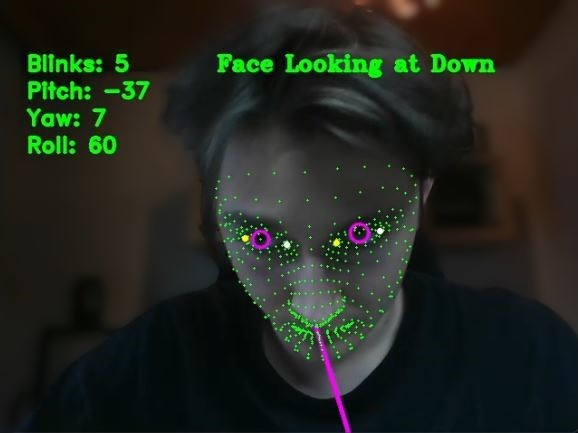
\includegraphics[scale=0.4]{old_tracker_face_gaze_webcam}
	\captionof{figure}{Ausgabe des Face-Gaze-Trackers, Quelle: \cite{lit_code_github_facegazetracker}} \label{fig:old_tracker_face_gaze_webcam}
\end{center}

<<<<<<< HEAD
=======
Eine weitere Option stellt das open source Projekt "Eyegaze Tracker" dar. Diese Software erfasst nicht die Gesichtsausrichtung, sondern die Pupillen. Dadurch kann sie Aussagen über die grobe Blickrichtung treffen. So wie in Abbildung \ref{fig:old_tracker_eyegaze_webcam} zu erkennen ist, kann bspw. die Aussage getroffen werden, dass die Testperson nach links schaut. Auch hier wird keine Blickposition auf dem Bildschirm geschätzt. Allerdings werden die Pupillen erfasst und die grobe Blickrichtung bestimmt. Die Blickposition kann gegebenenfalls mit den vorhandenen Daten durch eine Weiterentwicklung des vorhandenen open source Codes bestimmt werden. Dies würde allerdings einen erheblichen Entwicklungsaufwand bedeuten. 
>>>>>>> fd0befd8e95e2bae230d21ece8a1862eada6b577

Die Software schätzt nicht die Blickposition der Testperson auf dem Bildschirm, sondern gibt nur an, in welcher Lage sich der Kopf befindet. Diese Daten könnten aber als Grundlage für eine Weiterentwicklung dienen. Da allerdings nur die Ausrichtung des Gesichts und nicht der Pupillen in die Ausgabe einfließt, werden keine genauen Ergebnisse durch diese Herangehensweise erwartet.

<<<<<<< HEAD

Eine weitere Option stellt das open source Projekt 'Eyegaze Tracker' dar. Diese Software erfasst nicht die Gesichtsausrichtung, sondern die Pupillen. Dadurch kann sie eine qualitative Aussage über die Blickrichtung treffen. So wie in Abbildung \ref{fig:old_tracker_eyegaze_webcam} zu erkennen ist, kann bspw. die Aussage getroffen werden, dass die Testperson nach links schaut. Auch hier wird keine Blickposition auf dem Bildschirm geschätzt. Allerdings werden die Pupillen erfasst und die grobe Blickrichtung bestimmt. Die Blickposition kann gegebenenfalls mit den vorhandenen Daten durch eine Weiterentwicklung des vorhandenen open source Codes bestimmt werden. Dies würde allerdings einen erheblichen Entwicklungsaufwand bedeuten. 


\begin{center}
	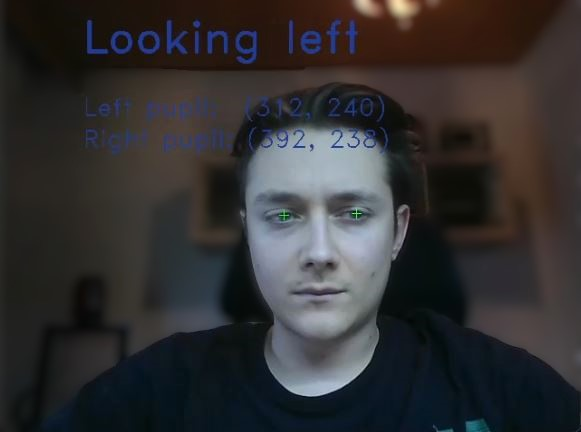
\includegraphics[scale=0.4]{old_tracker_eyegaze_webcam}
	\captionof{figure}{Ausgabe des Eyegaze-Trackers, Quelle: \cite{lit_code_github_gazetracking}} \label{fig:old_tracker_eyegaze_webcam}
\end{center}


Neben den oben genannten Projekten wurden auch noch einige weitere auf ihre Einsetzbarkeit in diesem Projekt untersucht. Diese hatten größtenteils ähnliche Eigenschaften und Einschränkungen. Eye Tracker die einen größeren Funktionsumfang bieten, wie beispielsweise das System 'Tobii Eye Tracker' haben den Nachteil, dass sie einen, je nach Budget, hohen finanziellen Aufwand bedeuten. Es wurde sich auf Grundlage umfangreicher Recherche und experimenteller Erprobung für den Beam Eye Tracker von Eyeware Tech entschieden. Dieser hat die in dieser Arbeit definierten Anforderungen erfüllt und soll als Basis für die weitere Entwicklung dienen.

\newpage

\section{Beam Eye Tracker}

Der Beam Eye Tracker ist für Gaming-Anwendungen und dem Einsatz von einfacher Hardware wie normalen Webcams entwickelt. Neben der Schätzung der Blickposition auf einen Punkt auf dem Bildschirm verfügt das Programm über eine Kopfpositionserkennung. Durch die Funktion 'Gaming Erweiterungen' teilt der Beam Eye Tracker die Trackingdaten über seine {\ac{API}} mit anderen Programmen.

Die Beam {\ac{API}} kann über die Programmiersprachen C++, C, C\# und Python angesprochen werden \cite{lit_code_beam_sdk}. Im Rahmen dieser Projektarbeit wird die {\ac{API}} mit Pyhton angesprochen. Verschiedene Klassen in der {\ac{API}} ermöglichen eine individuelle Einbindung der Eye Tracking Daten in eine selbst entwickelte Anwendung. Relevant für diese Projektarbeit ist die Klasse \glqq{}screen\_gaze\_info\grqq{}. Diese beinhaltet die x- und y- Koordinaten und die Angaben, ob die Augen erkannt werden und wie gut die Schätzung ist.

Durch die anwenderfreundliche {\ac{API}} des Beam {\ac{SDK}} und den niedrigen Preis von 29,99€ des Eye Trackers, fiel die Entscheidung, diesen für das Projekt zu nutzen. In Rücksprache mit den Beam-Entwicklern wurde der Beam Eye Tracker für dieses Projekt unentgeltlich zur Verfügung gestellt.
=======
Neben den oben genannten Projekten wurden auch noch einige weitere auf ihre Einsetzbarkeit in diesem Projekt untersucht. Diese hatten größtenteils ähnliche Eigenschaften und Einschränkungen. Eye Tracker die einen größeren Funktionsumfang bieten wie beispielsweise das System "Tobii Eye Tracker" haben den Nachteil, dass sie einen,je nach Budget, hohen finanziellen Aufwand bedeuten. Es wurde sich auf Grundlage umfangreicher Recherche und experimenteller Erprobung für den Beam Eye Tracker von Eyeware Tech entschieden. Dieser hat die in dieser Arbeit definierten Anforderungen erfüllt und soll als Basis für die weitere Entwicklung dienen.

\section{Beam Eye Tracker}

Der Beam Eye Tracker ist für Gaming-Anwendungen und dem Einsatz von einfacher Hardware wie normalen Webcams entwickelt. Neben der Schätzung der Blickposition auf einen Punkt auf dem Bildschirm verfügt das Programm über eine Kopfpositionserkennung. Durch die Funktion "Gaming Erweiterungen" teilt der Beam Eye Tracker die Trackingdaten mit anderen Programmen. Diese {\ac{API}} ermöglicht die Nutzung der Trackingdaten in eigenen Programmen. 

Die Beam {\ac{API}} kann über die Programmiersprachen C++, C, C\# und Python angesprochen werden \cite{lit_code_beam_sdk}. Im Rahmen dieser Projektarbeit wird die {\ac{API}} mit Pyhton angesprochen. Verschiedene Klassen in der {\ac{API}} ermöglichen eine individuelle Einbindung der Eye Tracking Daten in eine selbst entwickelte Anwendung. Relevant für diese Projektarbeit ist die Klasse \glqq{}screen\_gaze\_info\grqq{}. Diese beinhaltet die x- und y- Koordinaten und die Angaben, ob die Augen erkannt werden und wie gut die Schätzung ist.

Durch die anwenderfreundlichen {\ac{API}} des Beam {\ac{SDK}} und dem niedrigen Preis von 29,99€ des Eye Trackers fiel die Entscheidung, diesen für das Projekt zu nutzen. In Rücksprache mit den Beam Entwicklern wurde der Beam Eye Tracker für dieses Projekt unentgeltlich zur Verfügung gestellt.
>>>>>>> fd0befd8e95e2bae230d21ece8a1862eada6b577

	\chapter{Implementierung Eye Tracker}
\label{sec:implementierung eye tracker}

\section{Einrichtung im Fahrsimulator}

<<<<<<< HEAD
Eyeware Tech hat ihren Beam Eye Tracker so aufgebaut, dass er mit handelsüblicher Hardware verwendet werden kann. Das System kann bereits mit einer handelsüblichen {\ac{USB}} Webcam oder mit einer an den Computer angeschlossenen Smartphone-Kamera eingesetzt werden. Damit die Integration des Eye Trackers in den Fahrsimulator gelingt, müssen mehrere Voraussetzungen geschaffen werden. Diese werden in den folgenden Abschnitten beschrieben. 

Die Positionierung der Kamera ist von zentraler Bedeutung. Diese soll laut Eyeware Tech mittig zum Bildschirm ausgerichtet sein \cite{lit_software_beam_eyetracker}. Die Sitzposition der Testperson hingegen muss nicht mittig zur Kamera sein. Die Testperson kann auch relativ zur Kamera links oder rechts sitzen. Diese Annahme konnte durch selbst durchgeführte Tests bestätigt werden. 
In den Eye Tracker Einstellungen müssen auch die Kameraposition und der Neigungswinkel korrekt eingestellt werden. Die genauesten Ergebnisse konnten erzielt werden, als die Kamera im Fahrsimulator mittig zur Leinwand in der Mitte des Armaturenbretts angebracht war. Die Kameraposition wurde im Eye Tracker als 'unten' und mit einem Neigungswinkel von 0° angegeben.

Grundlage für verlässliche Ergebnisse ist es, die Kalibrierung, welche der Beam Eye Tracker integriert hat, vor jeder Sitzung im Fahrsimulator durchzuführen. Insbesondere wenn mehrere Personen nacheinander fahren, die sich von ihrer Körpergröße stark unterscheiden. Die in den Beam Eye Tracker integrierte Kalibrierung besteht aus fünf Punkten, die nacheinander auf der Leinwand erscheinen. Vier Punkte werden dabei in die vier Ecken der Leinwand positioniert. Der fünfte Punkt befindet sich in der Mitte der Leinwand. Während der Kalibrierung blickt die Testperson nacheinander auf diese Punkte. Sofern die Testperson einen Punkt fest fokussiert hat, klickt sie mit der Maus auf diesen Punkt. Der Eye Tracker verknüpft dann die aktuelle Blickposition mit den Koordinaten des Punktes auf der Leinwand. Nach diesem Prinzip kalibriert sich der Eye Tracker selbst und verknüpft die Position der Pupillen mit einer Position auf der Leinwand. Wie dieser Kalibrierungsprozess im Detail funktioniert, ist nicht bekannt.

Für die Tests des Eye Trackers wurde der mittelgroße Fahrsimulator in der {\ac{HKA}} eingesetzt. Da die Leinwand sehr groß ist und das Kalibrierungsfenster des Eye Trackers nicht verkleinert werden kann, befinden sich die Kalibrierungspunkte teilweise so weit in den Ecken, dass sie vor allem unten nicht mehr auf der Leinwand angezeigt werden. Das erschwert eine präzise Interaktion. Außerdem sollten während der Kalibrierung keine großen Kopfbewegungen gemacht werden. Experimente zeigten, dass das die Tracking-Genauigkeit verringern kann. Da die Punkte durch die breite Leinwand aber außerhalb des Sichtfelds der Testperson liegen, muss diese zwangsweise eine Kopfbewegung machen. 

Eine Herangehensweise, um diese Probleme zu minimieren, ist es, die Kalibrierung immer zu zweit durchzuführen. Die Testperson ist dafür verantwortlich, auf die Kalibrierungspunkte zu schauen und die zweite Person klickt auf diese mit der Maus. Da die Punkte teilweise außerhalb des Sichtfeldes liegen und die Testperson den Kopf nicht zu sehr bewegen sollte, ist es am besten, wenn diese nicht direkt auf den jeweiligen Punkt schaut, sondern leicht daneben. Wenn der Punkt bspw. unten rechts im Eck erscheint, dann richtet die Testperson bei der Kalibrierung ihren Blick leicht versetzt nach links. Zum einen wird dadurch die Kalibrierung insgesamt verbessert, da der Kopf nicht bewegt werden muss. Zusätzlich wird dadurch ein Fehler leicht abgeschwächt, welcher durch die Krümmung der Leinwand entsteht.

Zwischenzeitlich wurde im Rahmen dieser Projektarbeit auch der Ansatz einer eigenen Kalibrierung verfolgt. Diese hat vorausgesetzt, dass der Eye Tracker bereits einmal sehr grob mit dem integrierten Kalibrierungsfenster von Beam kalibriert wurde. Bei jedem Start des Programms wurde das selbst erstellte Kalibrierungsfenster geöffnet. Allerdings war das selbst entwickelte Kalibrierungsfenster in seiner Größe anpassbar. Dadurch wurden die Punkte im Sichtfeld der Testperson angezeigt und nicht an den Rändern der Leinwand. Eine schematische Abbildung des Kalibrierungsfensters ist in Abbildung \ref{fig:eigenes_kalibrierungsfenster} zu sehen. In der Realität hatte das Fenster einen weißen Hintergrund, um die Lichtverhältnisse relativ zum Beam Kalibrierungsfenster, welches sehr dunkel ist, zu verbessern. Die Ergebnisse der Kalibrierung wurden anschließend verwendet, um die Rohdaten des Eye Trackers mit diesen zu transformieren, damit die Kalibrierung Einfluss auf die Schätzwerte der Blickposition nimmt. Die daraus resultierenden Ergebnisse wiesen allerdings keine visuell erkennbare Verbesserung auf. Auf Basis der bisherigen Ergebnisse wird daher empfohlen, die integrierte Standard-Kalibrierung des Eye Trackers zu verwenden. Der Code für die selbst entwickelte Kalibrierung ist allerdings weiterhin in auskommentierter Form vorhanden und kann bei Bedarf wieder reaktiviert und weiterentwickelt werden. 
=======
Eyeware Tech hat ihren Beam Eye Tracker so aufgebaut, dass er mit handelsüblicher Hardware verwendet werden kann. Das System kann bereits mit einer handelsüblichen {\ac{USB}} Webcam oder mit einer an den Computer angeschlossenen Smartphone-Kamera eingesetzt werden. Damit die Integration des Eye Trackers in den Fahrsimulator gelingt, müssen einige Punkte beachtet werden. 

Die Positionierung der Kamera ist von zentraler Bedeutung. Diese soll lauf Eyeware Tech mittig zum Bildschirm ausgerichtet sein \cite{lit_software_beam_eyetracker}. Die Sitzposition der Testperson hingegen muss nicht mittig zur Kamera sein. Die Testperson kann auch relativ zur Kamera weiter links oder weiter rechts sitzen. Diese Annahme konnte durch selbst durchgeführte Tests bestätigt werden. 
In den Eye Tracker Einstellungen muss auch die Kameraposition und der Neigungswinkel korrekt eingestellt werden. Die genauesten Ergebnisse konnten erzielt werden, als die Kamera im Fahrsimulator mittig auf dem Display in der Mitte des Armaturenbretts angebracht war. Die Kameraposition wurde im Eye Tracker als "unten" und mit einem Neigungswinkel von 0° angegeben.

Grundlage für verlässliche Ergebnisse ist es die Kalibrierung, welche der Beam Eye Tracker integriert hat, vor jeder Sitzung im Fahrsimulator durchzuführen. Insbesondere wenn mehrere Personen nacheinander fahren, die sich von ihrer Körpergröße stark unterscheiden. Die in den Beam Eye Tracker integrierte Kalibrierung besteht aus fünf Punkten, die nacheinander auf der Leinwand erscheinen. Vier Punkte werden dabei in die vier Ecken der Leinwand positioniert. Der fünfte Punkt befindet sich in der Mitte der Leinwand. Während der Kalibrierung blickt die Testperson nacheinander auf diese Punkte. Sofern die Testperson einen Punkt fest fokussiert hat, klickt sie mit der Maus auf diesen Punkt. Der Eye Tracker verknüpft dann die aktuelle Blickposition mit den Koordinaten des Punktes auf der Leinwand. Nach diesem Prinzip kalibriert sich der Eye Tracker selbst und verknüpft die Position der Pupillen mit einer Position auf der Leinwand. Wie dieser Kalibrierungsprozess im Detail funktioniert ist nicht bekannt.

Für die Tests des Eye Trackers wurde der mittelgroße Fahrsimulator in der {\ac{HKA}} eingesetzt. Da die Leinwand sehr groß ist und das Kalibrierungsfenster des Eye Trackers nicht verkleinert werden kann, befinden sich die Kalibrierungspunkte teilweise so weit in den Ecken, dass sie vor allem unten nicht mehr auf der Leinwand angezeigt werden. Das erschwert eine präzise Interaktion. Außerdem sollten während der Kalibrierung keine großen Kopfbewegungen gemacht werden. Experimente zeigten, dass das die Tracking Genauigkeit verringern kann. Da die Punkte durch die breite Leinwand aber außerhalb des Sichtfelds der Testperson liegen, muss diese zwangsweise eine Kopfbewegung machen. 

Eine Herangehensweise um diese Probleme zu minimieren ist es, die Kalibrierung immer zu zweit durchzuführen. Die Testperson ist dafür verantwortlich auf die Kalibrierungspunkte zu schauen und die zweite Person klickt auf diese mit der Maus. Da die Punkte teilweise außerhalb des Sichtfeldes liegen und die Testperson den Kopf nicht zu sehr bewegen sollte, ist es am besten, wenn diese nicht direkt auf den jeweiligen Punkt schaut, sondern leicht daneben. Wenn der Punkt bspw. unten rechts im Eck erscheint, dann richtet die Testperson bei der Kalibrierung ihren Blick leicht versetzt nach links. Zum einen wird dadurch die Kalibrierung insgesamt verbessert, da der Kopf nicht bewegt werden muss. Zusätzlich wird dadurch ein Fehler leicht abgeschwächt, welcher durch die Krümmung der Leinwand entsteht.
Zwischenzeitlich wurde im Rahmen dieser Projektarbeit auch der Ansatz einer eigenen Kalibrierung verfolgt. Diese hat vorausgesetzt, dass der Eye Tracker bereits einmal sehr grob mit dem integrierten Kalibrierungsfenster von Beam kalibriert wurde. Bei jedem Start des Programms wurde das selbst erstellte Kalibrierungsfenster geöffnet. Allerdings war das selbst entwickelte Kalibrierungsfenster in seiner Größe anpassbar. Dadurch wurden die Punkte im Sichtfeld der Testperson angezeigt und nicht an den Rändern der Leinwand. Eine schematische Abbildung des Kalibrierungsgfensters ist in Abbildung \ref{fig:eigenes_kalibrierungsfenster} zu sehen. In der Realität hatte das Fenster einen weißen Hintergrund, um die Lichtverhältnisse relativ zum Beam Kalibrierungsfenster, welches sehr dunkel ist, zu verbessern. Die Ergebnisse der Kalibrierung wurden anschließend verwendet, um die Rohdaten des Eye Trackers mit diesen zu transformieren, damit die Kalibrierung Einfluss auf die Schätzwerte der Blickposition nimmt. Die daraus resultierten Ergebnisse wiesen allerdings keine wirkliche Verbesserung auf. Auf Basis der bisherigen Ergebnisse wird daher empfohlen die integrierte Standard-Kalibrierung des Eye Trackers zu verwenden. Der Code für die selbst entwickelte Kalibrierung ist allerdings weiterhin in auskommentierter Form vorhanden und kann bei Bedarf wieder reaktiviert und weiterentwickelt werden. 

\begin{figure}[h]
	\begin{center}
		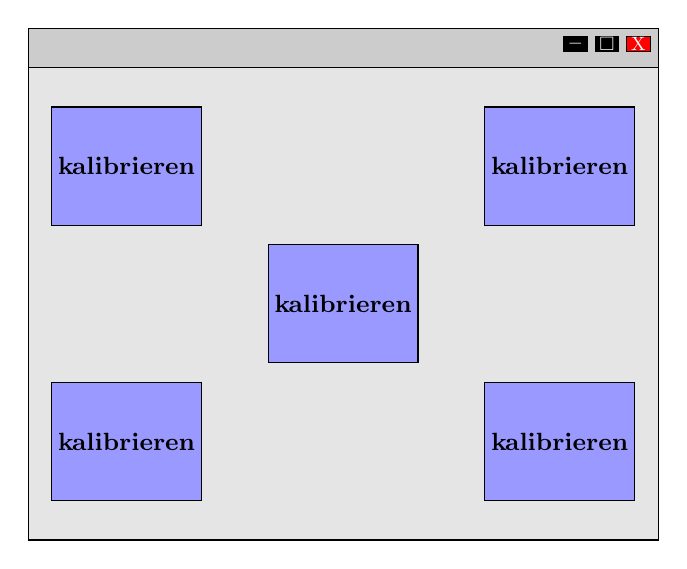
\begin{tikzpicture}[scale=1]
			% Fensterhintergrund
			\draw[fill=gray!20] (0,0) rectangle (8,6);
			
			% Fensterleiste mit Min, Max, Schließen
			\draw[fill=gray!40] (0,6) rectangle (8,6.5);
			\draw[fill=black] (6.8,6.2) rectangle (7.1,6.4); % Minimieren
			\draw[fill=black] (7.2,6.2) rectangle (7.5,6.4); % Maximieren
			\draw[fill=red] (7.6,6.2) rectangle (7.9,6.4); % Schließen
			\node at (6.95,6.3) {\textcolor{white}{\scalebox{0.7}{$-$}}};
			\node at (7.35,6.3) {\textcolor{white}{\scalebox{0.7}{$\square$}}};
			\node at (7.75,6.3) {\textcolor{white}{\scalebox{0.7}{X}}};
			
			% Kalibrierungsknöpfe
			\draw[fill=blue!40] (0.3,0.5) rectangle (2.2,2); % Unten links
			\draw[fill=blue!40] (5.8,0.5) rectangle (7.7,2); % Unten rechts
			\draw[fill=blue!40] (0.3,4) rectangle (2.2,5.5); % Oben links
			\draw[fill=blue!40] (5.8,4) rectangle (7.7,5.5); % Oben rechts
			\draw[fill=blue!40] (3.05,2.25) rectangle (4.95,3.75); % Mitte
			
			% Text auf den Knöpfen
			\node at (1.25,1.25) {\small \textbf{kalibrieren}};
			\node at (6.75,1.25) {\small \textbf{kalibrieren}};
			\node at (1.25,4.75) {\small \textbf{kalibrieren}};
			\node at (6.75,4.75) {\small \textbf{kalibrieren}};
			\node at (4,3) {\small \textbf{kalibrieren}};
		\end{tikzpicture}
	\end{center}
	\caption{Schematische Darstellung des selbst entwickelten Kalibrierungsfensters}\label{fig:eigenes_kalibrierungsfenster}
\end{figure}


Während der Kalibrierung und der gesamten Verwendung des Eye Tracking Systems darf ausschließlich die Testperson im Fahrsimulator sitzen. Eine zweite Person würde das Tracking System beeinflussen, da nicht selektiert werden kann, welche Augen getrackt werden sollen und welche nicht. In Zukunft muss hier eine visuelle Abschirmung, wie eine Art Scheuklappe eingebaut werden, um dieses Problem zu lösen. 

Ein weiterer wichtiger Faktor ist die Beleuchtung im Fahrsimulator. Das Kalibrierungsfenster des Beam Eye Trackers hat einen schwarzen Hintergrund. Wenn keine externe Lichtquelle verwendet wird, dann sind die Lichtverhältnisse unzureichend, als dass eine ordentliche Kalibrierung stattfinden könnte. Selbst wenn während der Kalibrierung gute Lichtverhältnisse herrschen, reicht die Helligkeit der Leinwand allein während des Fahrens nicht aus, um verlässliche Ergebnisse zu liefern. Es konnte eine deutliche Verbesserung der Trackingqualität erzielt werden, nachdem im Fahrsimulator eine externe Lichtquelle während der gesamten Kalibrierung und der gesamten Fahrzeit eingesetzt wurde. 
Neben externen Mitteln, um die Lichtverhältnisse zu verbessern, können auch in der Windows Kamera App Anpassungen vorgenommen werden. Dazu muss in den Einstellungen der Kamera App unter "Kameraeinstellungen" die Option "Erweiterte Steuerelemente für Fotos und Videos" aktiviert werden. Dadurch wird ein Helligkeitsregler verfügbar, der die Helligkeit des Kamerabildes systemweit verändert. Je nach aktuellen Lichtverhältnissen kann ein Erhöhen oder Verringern der Bildhelligkeit den Kontrast der Pupillen relativ zur Umgebung verbessern.

\begin{figure}[h!]
	\begin{center}
		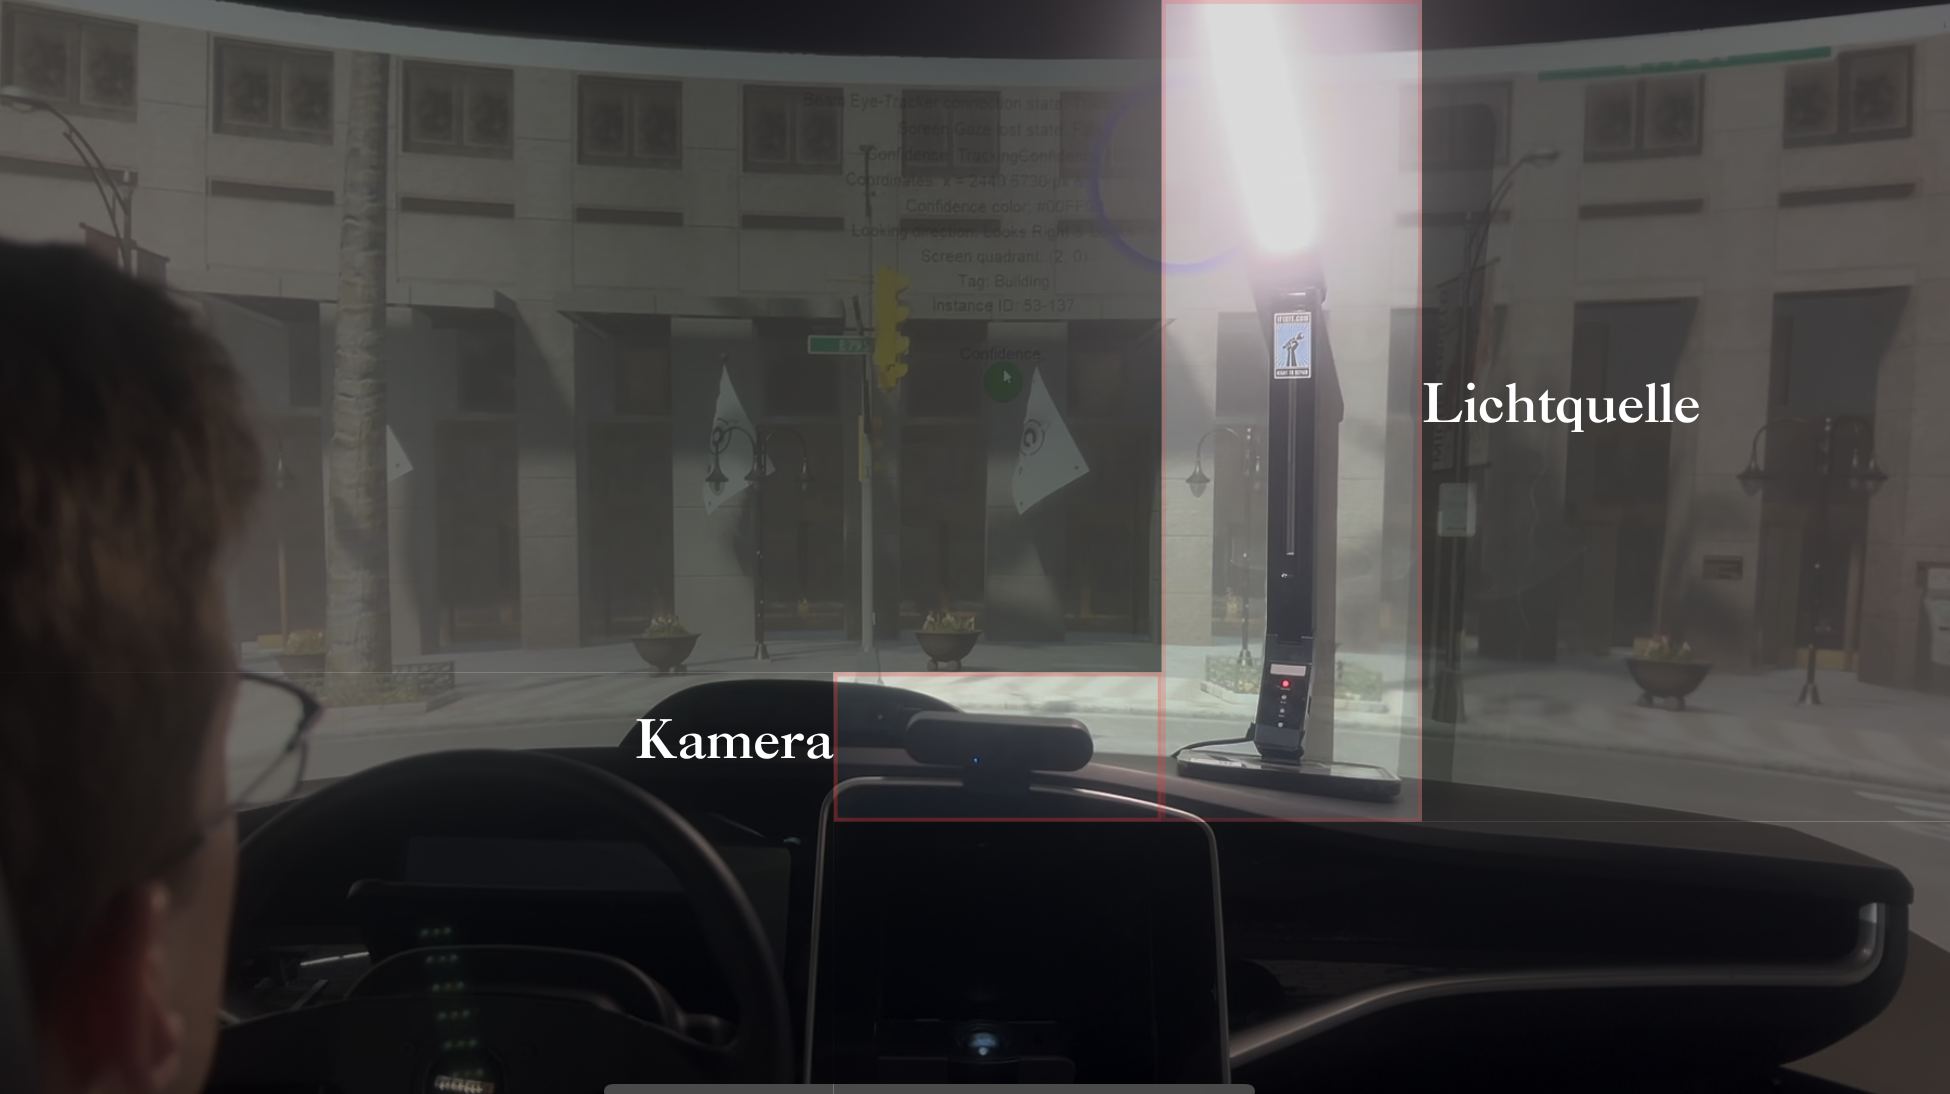
\includegraphics[scale=0.19]{camera_position}
		\caption{Positionierung von Kamera und externer Lichtquelle, Quelle: \cite{lit_software_canva}} \label{fig:camera_position}
	\end{center}
\end{figure}


In Abbildung \ref{fig:camera_position} sind die Kameraposition und die externe Lichtquelle aufgebaut im Fahrsimulator zu erkennen. Licht und Kamera sollten zu einem späteren Zeitpunkt noch besser in das System integriert werden. Zu Testzwecken hat der Aufbau allerdings verlässliche Ergebnisse geliefert. 
>>>>>>> fd0befd8e95e2bae230d21ece8a1862eada6b577



\begin{center}
	\resizebox{0.45\linewidth}{!}{
	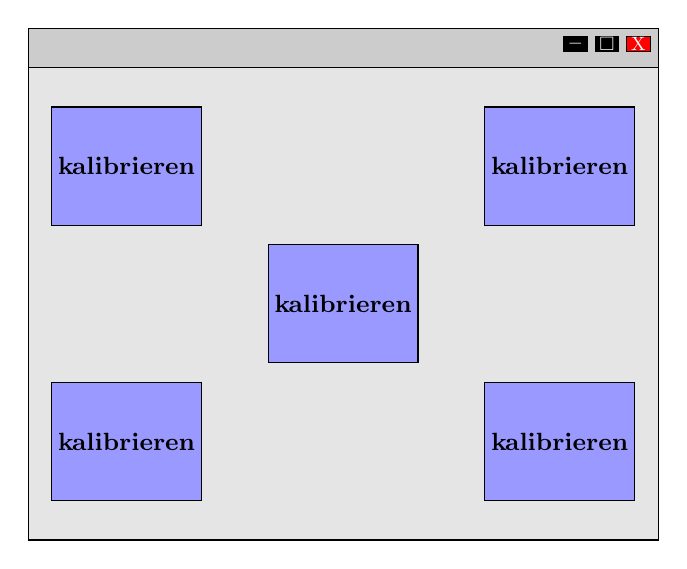
\begin{tikzpicture}[scale=1]
		% Fensterhintergrund
		\draw[fill=gray!20] (0,0) rectangle (8,6);
		
		% Fensterleiste mit Min, Max, Schließen
		\draw[fill=gray!40] (0,6) rectangle (8,6.5);
		\draw[fill=black] (6.8,6.2) rectangle (7.1,6.4); % Minimieren
		\draw[fill=black] (7.2,6.2) rectangle (7.5,6.4); % Maximieren
		\draw[fill=red] (7.6,6.2) rectangle (7.9,6.4); % Schließen
		\node at (6.95,6.3) {\textcolor{white}{\scalebox{0.7}{$-$}}};
		\node at (7.35,6.3) {\textcolor{white}{\scalebox{0.7}{$\square$}}};
		\node at (7.75,6.3) {\textcolor{white}{\scalebox{0.7}{X}}};
		
		% Kalibrierungsknöpfe
		\draw[fill=blue!40] (0.3,0.5) rectangle (2.2,2); % Unten links
		\draw[fill=blue!40] (5.8,0.5) rectangle (7.7,2); % Unten rechts
		\draw[fill=blue!40] (0.3,4) rectangle (2.2,5.5); % Oben links
		\draw[fill=blue!40] (5.8,4) rectangle (7.7,5.5); % Oben rechts
		\draw[fill=blue!40] (3.05,2.25) rectangle (4.95,3.75); % Mitte
		
		% Text auf den Knöpfen
		\node at (1.25,1.25) {\small \textbf{kalibrieren}};
		\node at (6.75,1.25) {\small \textbf{kalibrieren}};
		\node at (1.25,4.75) {\small \textbf{kalibrieren}};
		\node at (6.75,4.75) {\small \textbf{kalibrieren}};
		\node at (4,3) {\small \textbf{kalibrieren}};
	\end{tikzpicture}
}
\end{center}
\captionof{figure}{Schematische Darstellung des selbst entwickelten Kalibrierungsfensters}\label{fig:eigenes_kalibrierungsfenster}



Während der Kalibrierung und der gesamten Verwendung des Eye Tracking Systems darf ausschließlich die Testperson im Fahrsimulator sitzen. Eine zweite Person würde das Tracking System beeinflussen, da nicht selektiert werden kann, welche Augen getrackt werden sollen und welche nicht. In Zukunft muss hier eine visuelle Abschirmung, wie eine Art Scheuklappe eingebaut werden, um dieses Problem zu lösen.

Ein weiterer wichtiger Faktor ist die Beleuchtung im Fahrsimulator. Das Kalibrierungsfenster des Beam Eye Trackers hat einen schwarzen Hintergrund. Wenn keine externe Lichtquelle verwendet wird, dann sind die Lichtverhältnisse unzureichend, als dass eine ordentliche Kalibrierung stattfinden könnte. Selbst wenn während der Kalibrierung gute Lichtverhältnisse herrschen, reicht die Helligkeit der Leinwand während des Fahrens nicht aus, um verlässliche Ergebnisse zu liefern. Es konnte eine Verbesserung der Trackingqualität erzielt werden, nachdem im Fahrsimulator eine externe Lichtquelle während der gesamten Kalibrierung und der gesamten Fahrzeit eingesetzt wurde. 
Neben externen Mitteln, um die Lichtverhältnisse zu verbessern, können auch in der Windows Kamera App Anpassungen vorgenommen werden. Dazu muss in den Einstellungen der Kamera App unter 'Kameraeinstellungen' die Option 'Erweiterte Steuerelemente für Fotos und Videos' aktiviert werden. Dadurch wird ein Helligkeitsregler verfügbar, der die Helligkeit des Kamerabildes systemweit verändert. Je nach aktuellen Lichtverhältnissen kann ein Erhöhen oder Verringern der Bildhelligkeit den Kontrast der Pupillen relativ zur Umgebung verbessern.


\begin{center}
	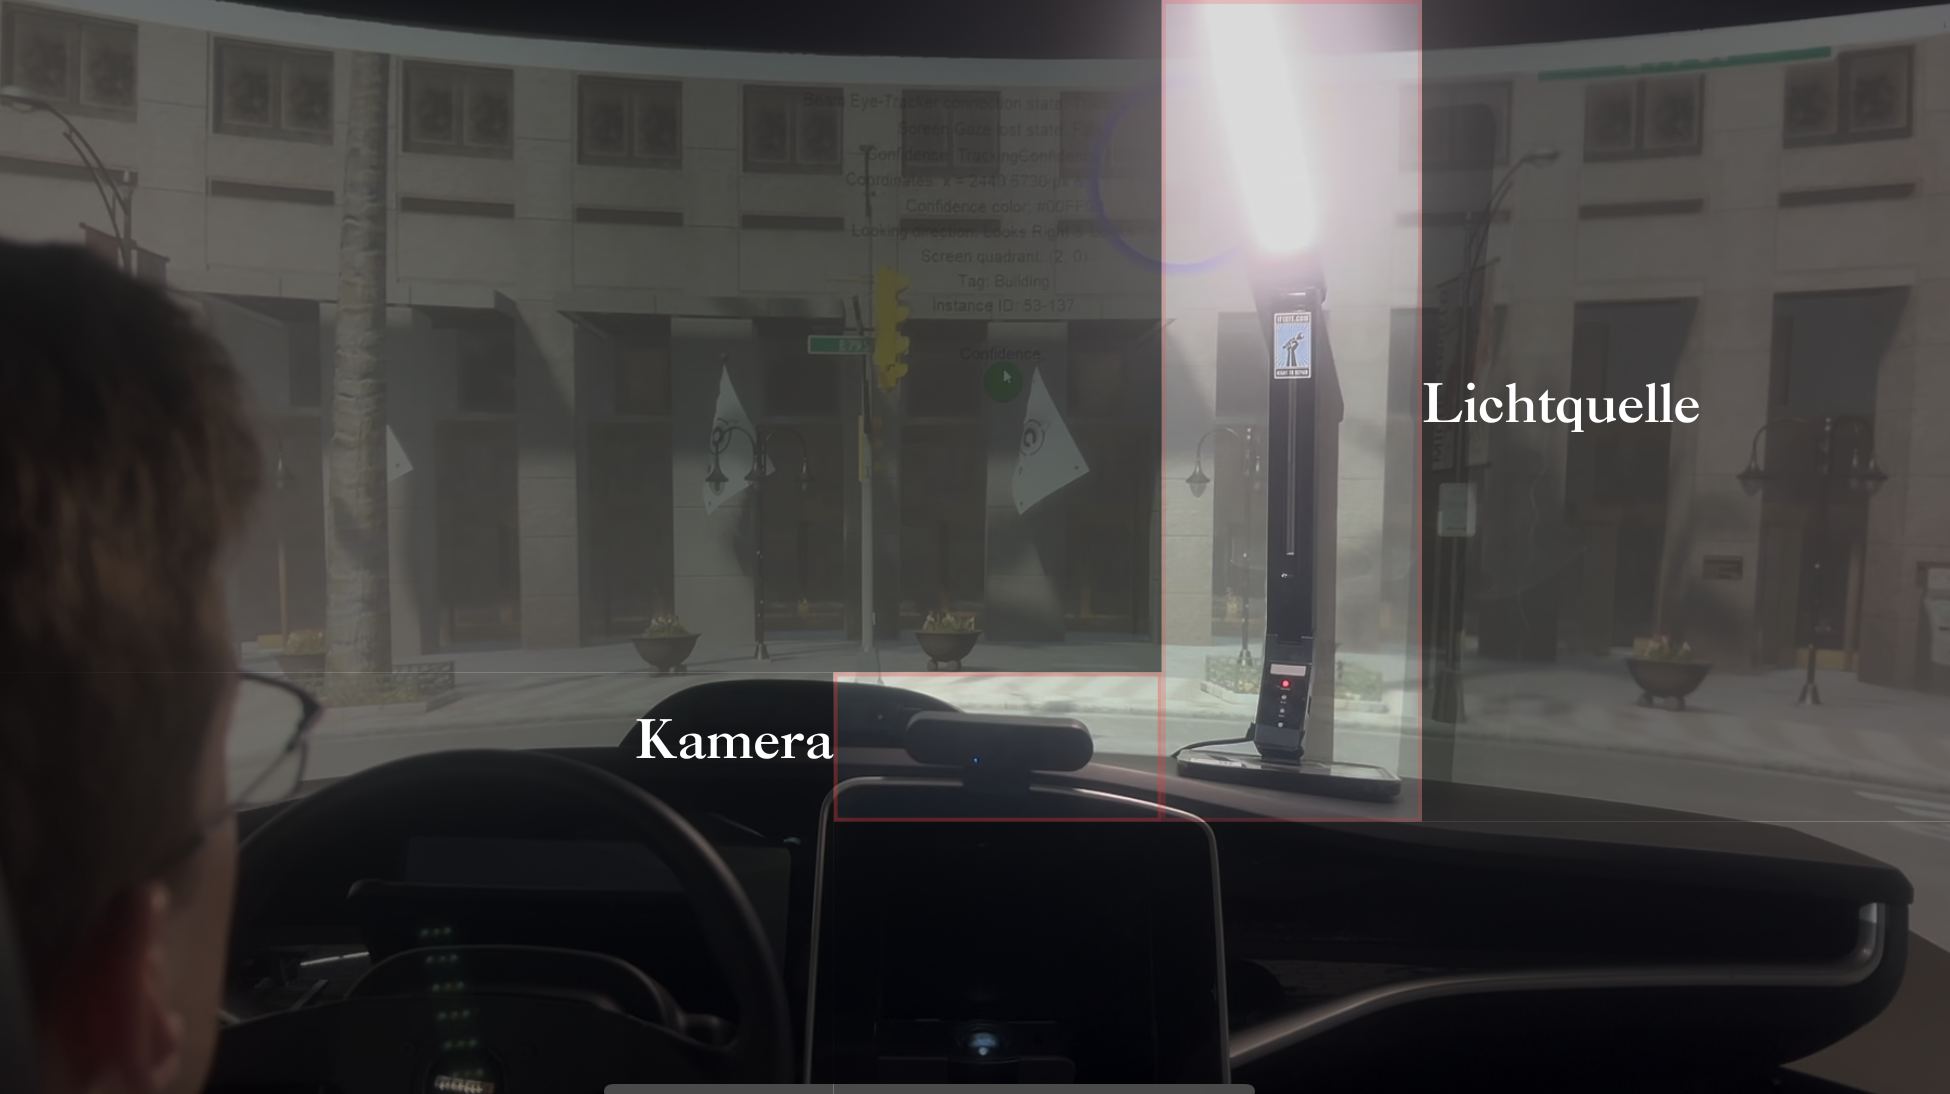
\includegraphics[scale=0.19]{camera_position}
	\captionof{figure}{Positionierung von Kamera und externer Lichtquelle, Quelle: \cite{lit_software_canva}} \label{fig:camera_position}
\end{center}



In Abbildung \ref{fig:camera_position} sind die Kameraposition und die externe Lichtquelle im Fahrsimulator zu erkennen. Licht und Kamera sollten zu einem späteren Zeitpunkt noch besser in das System integriert werden. Zu Testzwecken hat der Aufbau allerdings verlässliche Ergebnisse geliefert. 

\newpage

\section{Beam Eye Tracker SDK}
<<<<<<< HEAD
Eyewear Tech bietet beim Kauf des Beam Eye Tracker das {\ac{SDK}} an. Das {\ac{SDK}} ermöglicht es, die Ausgabe des Eye Trackers in selbst geschriebenen Anwendungen zu verwenden \cite{lit_website_beam_sdk_documentation}. Das {\ac{SDK}} muss nicht zusätzlich erworben werden, sondern ist im Kaufpreis des Eye Trackers enthalten.
Auf der Website des Beam {\ac{SDK}} wird in Python geschriebener Beispielcode zur Verfügung gestellt. In diesem Code werden die nötigen Schritte für eine Verbindung mit der {\ac{API}} des Eye Trackers durchgeführt. Der Code wurde auch als Grundlage für die Implementierung des Eye Trackers in dem Programm, das im Rahmen dieser Arbeit entwickelt wurde, verwendet \cite{lit_code_beam_sdk}.


\textsf{}
\begin{center}
	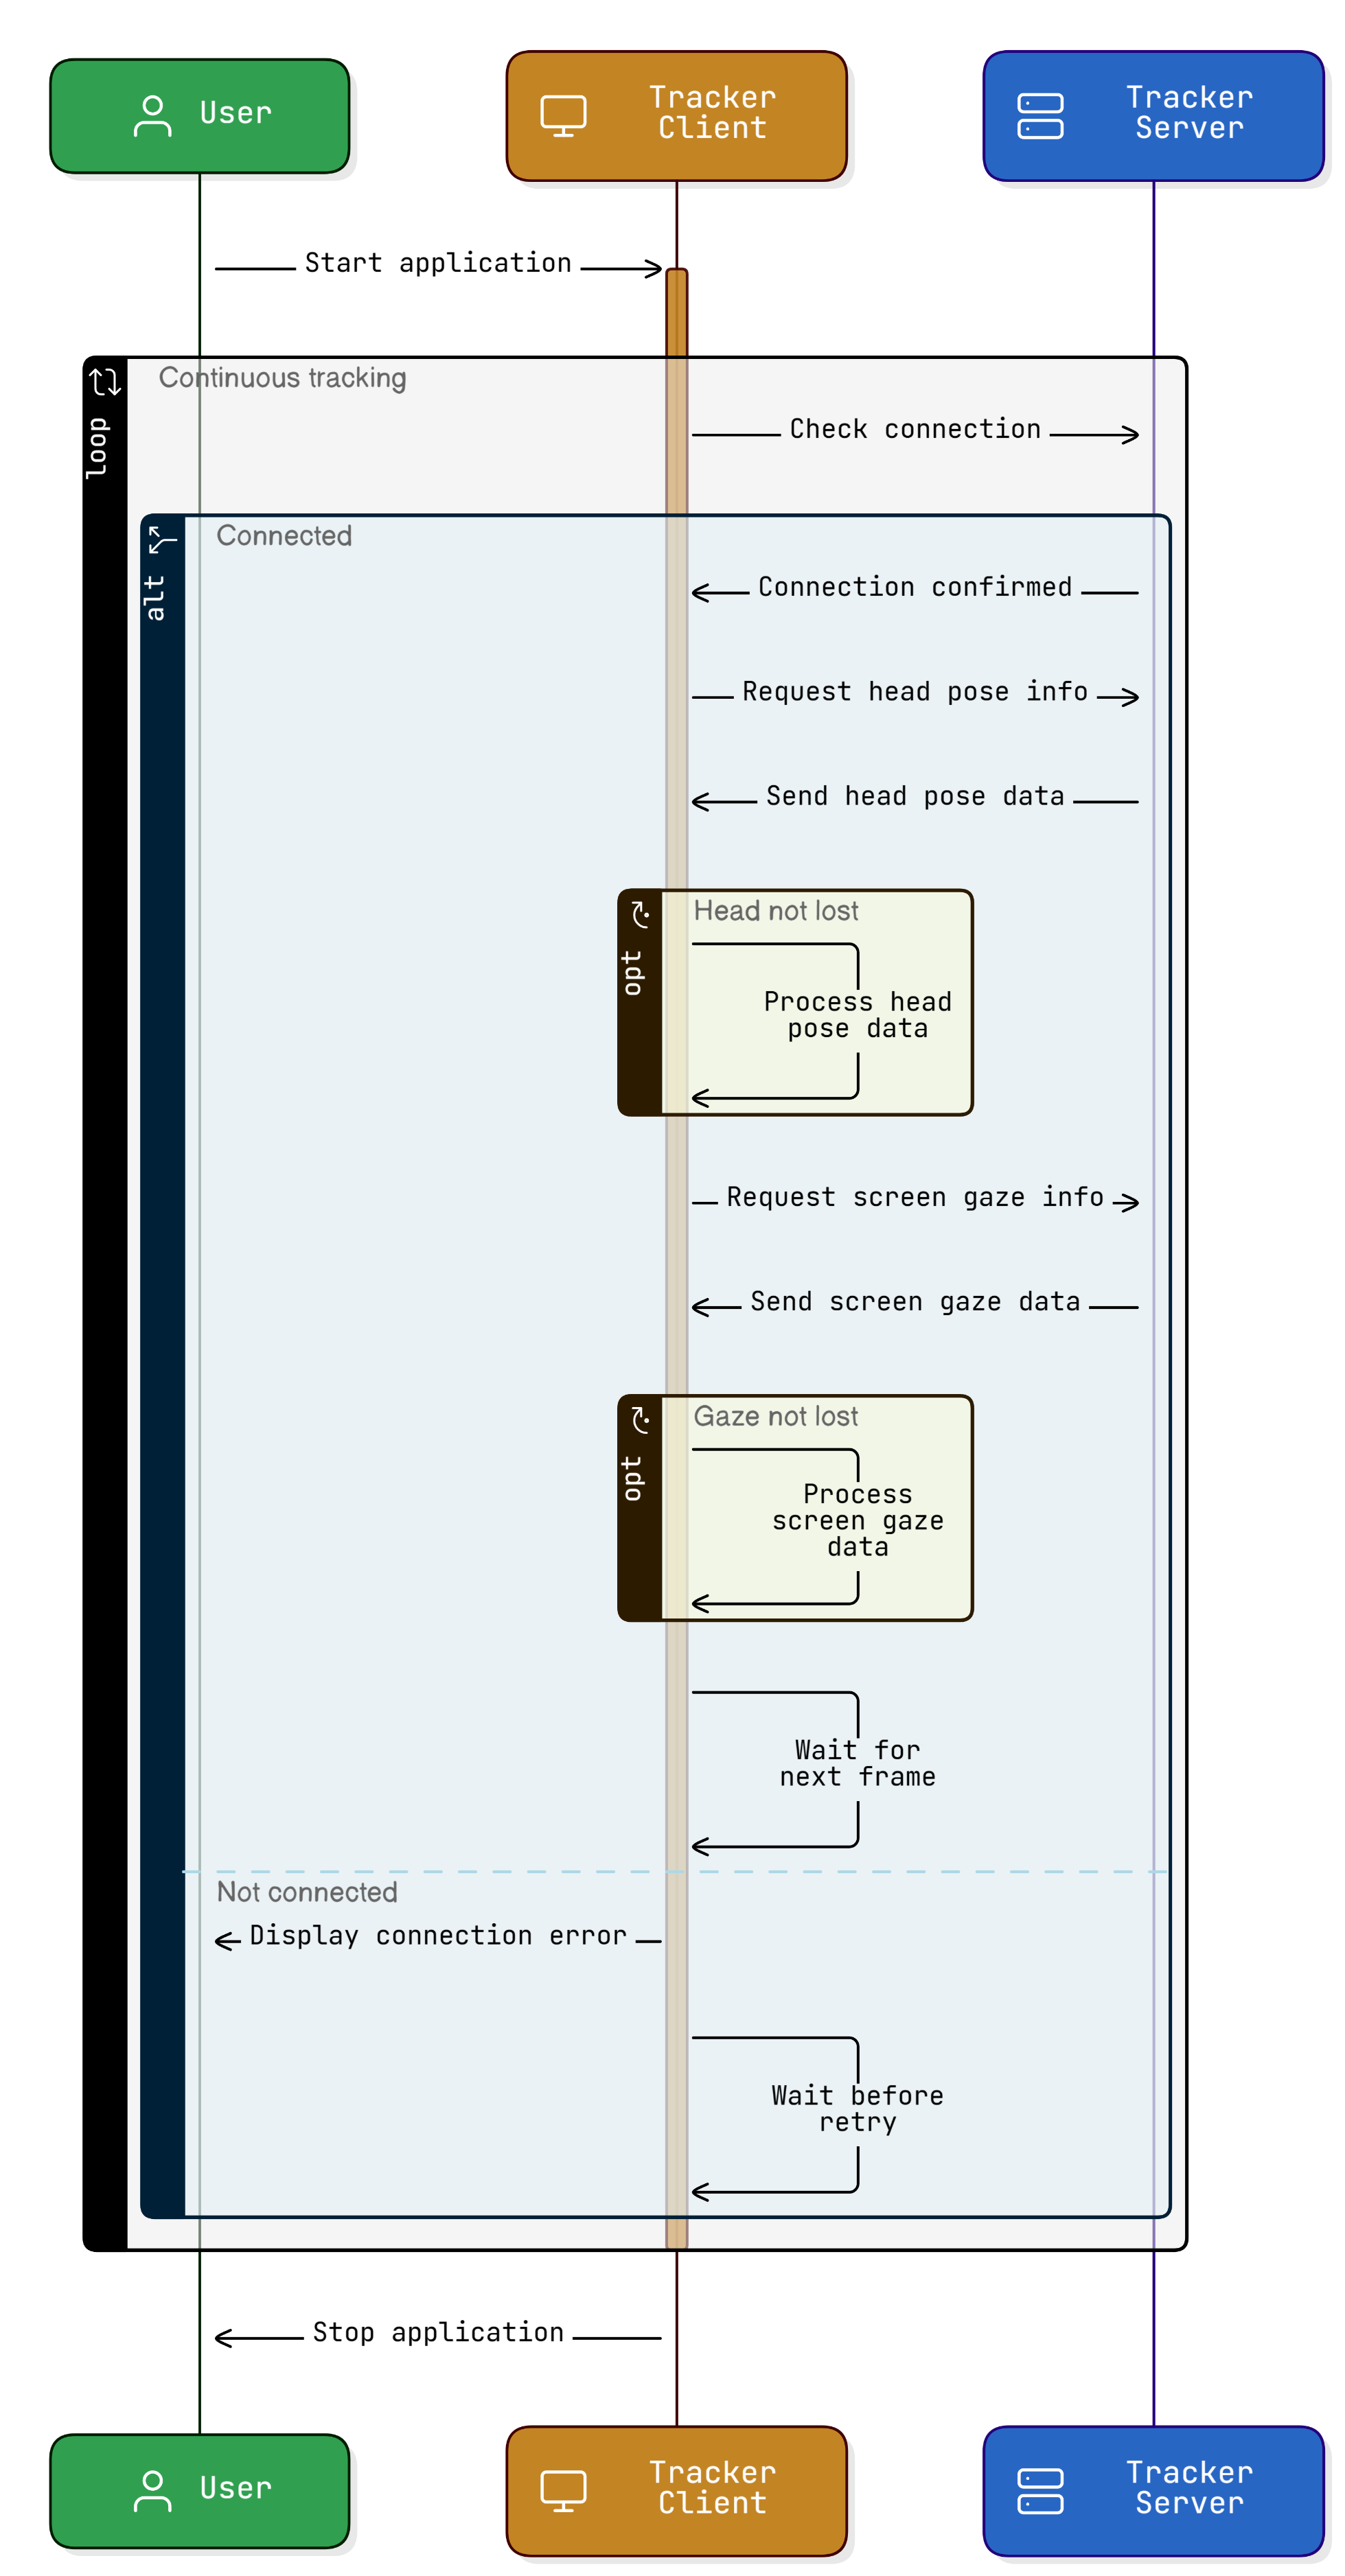
\includegraphics[scale=0.11]{code_structure_beam}
	\captionof{figure}{Visuelle Darstellung des Codes zur Beam {\ac{SDK}}, Quelle: nachempfunden: \cite{lit_code_beam_sdk}, \cite{lit_software_eraserio}} \label{fig:code_structure_beam}
\end{center}



Die Funktionsweise der {\ac{API}} ist vereinfacht in Abbildung \ref{fig:code_structure_beam} zu erkennen. Der Tracker Server ist die Bezeichnung für den Eye Tracker selbst. Der Client ist das selbst geschriebene Programm, welches die Trackerdaten über die {\ac{API}} entgegennimmt. Die beiden zentralen Informationen, welche vom Server an den Client übergeben werden, sind die Daten zur Kopfposition (head pose data) und die Daten zur Blickposition (screen gaze data). Die Kopfposition gibt Auskunft über die Translation und Rotation des Kopfes der Testperson. Die Blickposition gibt Auskunft darüber, auf welchen Punkt auf dem Bildschirm die Testperson schaut \cite{lit_website_beam_sdk_documentation}. Diese beiden Systeme laufen unabhängig voneinander und dienen unterschiedlichen Einsatzzwecken. Das Kopftracking kann bspw. dazu dienen, die Kamera in einer Simulationswelt zu bewegen. Das könnte Sinn machen, wenn keine große Leinwand wie im Fahrsimulator vorhanden ist. Durch einen Blick nach links könnte sich auch die Kamera im Fahrsimulator mit nach links bewegen. Für den Einsatzzweck im Fahrsimulator ist diese Funktion durch die große Leinwand allerdings nicht notwendig. Die Daten werden dennoch übermittelt, falls in Zukunft doch ein Anwendungsfall entstehen sollte. Die Gaze Daten stellen im Kontext dieser Arbeit die primär relevante Information dar. Diese geben eine Schätzung ab, auf welchen Punkt die Testperson auf der Leinwand schaut. Sofern eine Testperson vom Eye Tracker erkannt wird, werden in kontinuierlichen Abständen diese Daten vom Eye Tracker an den Client übermittelt. Zusätzlich dazu werden auch noch andere Daten wie bspw. die confidence übermittelt. Dabei handelt es sich um einen Wert, welcher mit jeder geschätzten Blickposition mit übermittelt wird. Dieser gibt an, wie sicher sich der Eye Tracker mit seiner Schätzung der aktuellen Blickposition ist \cite{lit_website_beam_sdk_documentation}. 

\section{Schnittstelle zu CARLA}

Im folgenden Abschnitt soll der Datenfluss zwischen CARLA und dem Eye Tracker sowie dem selbstgeschriebenen Programm erläutert werden.
Der Eye Tracker und CARLA arbeiten größtenteils getrennt voneinander. Die visuelle Ausgabe des Eye Trackers erfolgt durch einen kleinen schwarzen Punkt, welcher die aktuell geschätzte Blickposition auf der Leinwand anzeigt. Dieser schwarze Punkt befindet sich in einem selbst erstellten transparenten Fenster, welches über den Bildschirm gelegt wird. Der schwarze Punkt ist nicht Teil von CARLA oder dem Eye Tracker sondern wird durch das selbst geschriebene Programm erzeugt. Er basiert auf den x- und y-Koordinaten des Eye Trackers, welche durch eine zusätzliche Korrekturfunktion optimiert werden. Diese Korrektur wird in einem späteren Abschnitt genauer erläutert. Es gibt auch einen sogenannten Textmanager. Dieser ist auch selbst entwickelt und weder Teil von CARLA noch vom Beam Eye Tracker. In diesem werden für den Nutzer unter anderem die grobe Blickrichtung in Textform angezeigt. Zum Beispiel 'schaut nach oben links'. Der Text Manager, wird wie in der Abbildung \ref{fig:eye_tracker_data} zu sehen ist, mit Informationen des Eye Trackers und von CARLA gespeist.

Die einzige direkte Schnittstelle zwischen CARLA und den Daten des Eye Trackers ist die Übergabe der Eye Tracker Daten an die Auswertung des Instance Segmentation Sensors. Dieser Sensor wird in einem späteren Abschnitt genauer erläutert. Diese Schnittstelle ist in Abbildung \ref{fig:eye_tracker_data} schematisch dargestellt. Der CARLA Server sendet die Sensordaten des Instance Segmentation Sensors an den CARLA Client. Der CARLA Client übergibt die Sensordaten an die Auswertung. Bei der Auswertung werden die Rohdaten des Eye Trackers, die zuvor durch eine Krümmungs-Korrektur angepasst wurden, dann mit den Sensordaten des Instance Segmentation Sensors verarbeitet. Durch die Kombination aus Eye Tracking Daten und den Daten des Sensors kann eine Aussage darüber getroffen werden, auf welches Objekt die Testperson innerhalb der CARLA Simulationswelt schaut. Diese Ausgabe wird dann im Text Manager in Form von Text auf dem Bildschirm dargestellt. Eine genaue Beschreibung der Funktionsweise der einzelnen Elemente folgt in späteren Abschnitten.
=======
Eyewear Tech bietet beim Kauf des Beam Eye Tracker das {\ac{SDK}} an. Das {\ac{SDK}} ermöglicht es die Ausgabe des Eye Trackers in selbst geschriebenen Anwendungen zu verwenden \cite{lit_website_beam_sdk_documentation}. Das {\ac{SDK}} muss nicht zusätzlich erworben werden, sondern ist im Kaufpreis des Eye Trackers enthalten.
Auf der Website des Beam {\ac{SDK}} wird in Python geschriebener Beispielcode zur Verfügung gestellt. In diesem Code werden die nötigen Schritte für eine Verbindung mit der {\ac{API}} des Eye Trackers durchgeführt. Der Code wurde auch als Grundlage für die Implementierung des Eye Trackers in dem Programm, das im Rahmen dieser Arbeit entwickelt wurde verwendet \cite{lit_code_beam_sdk}.


\begin{figure}[h!]
	\begin{center}
		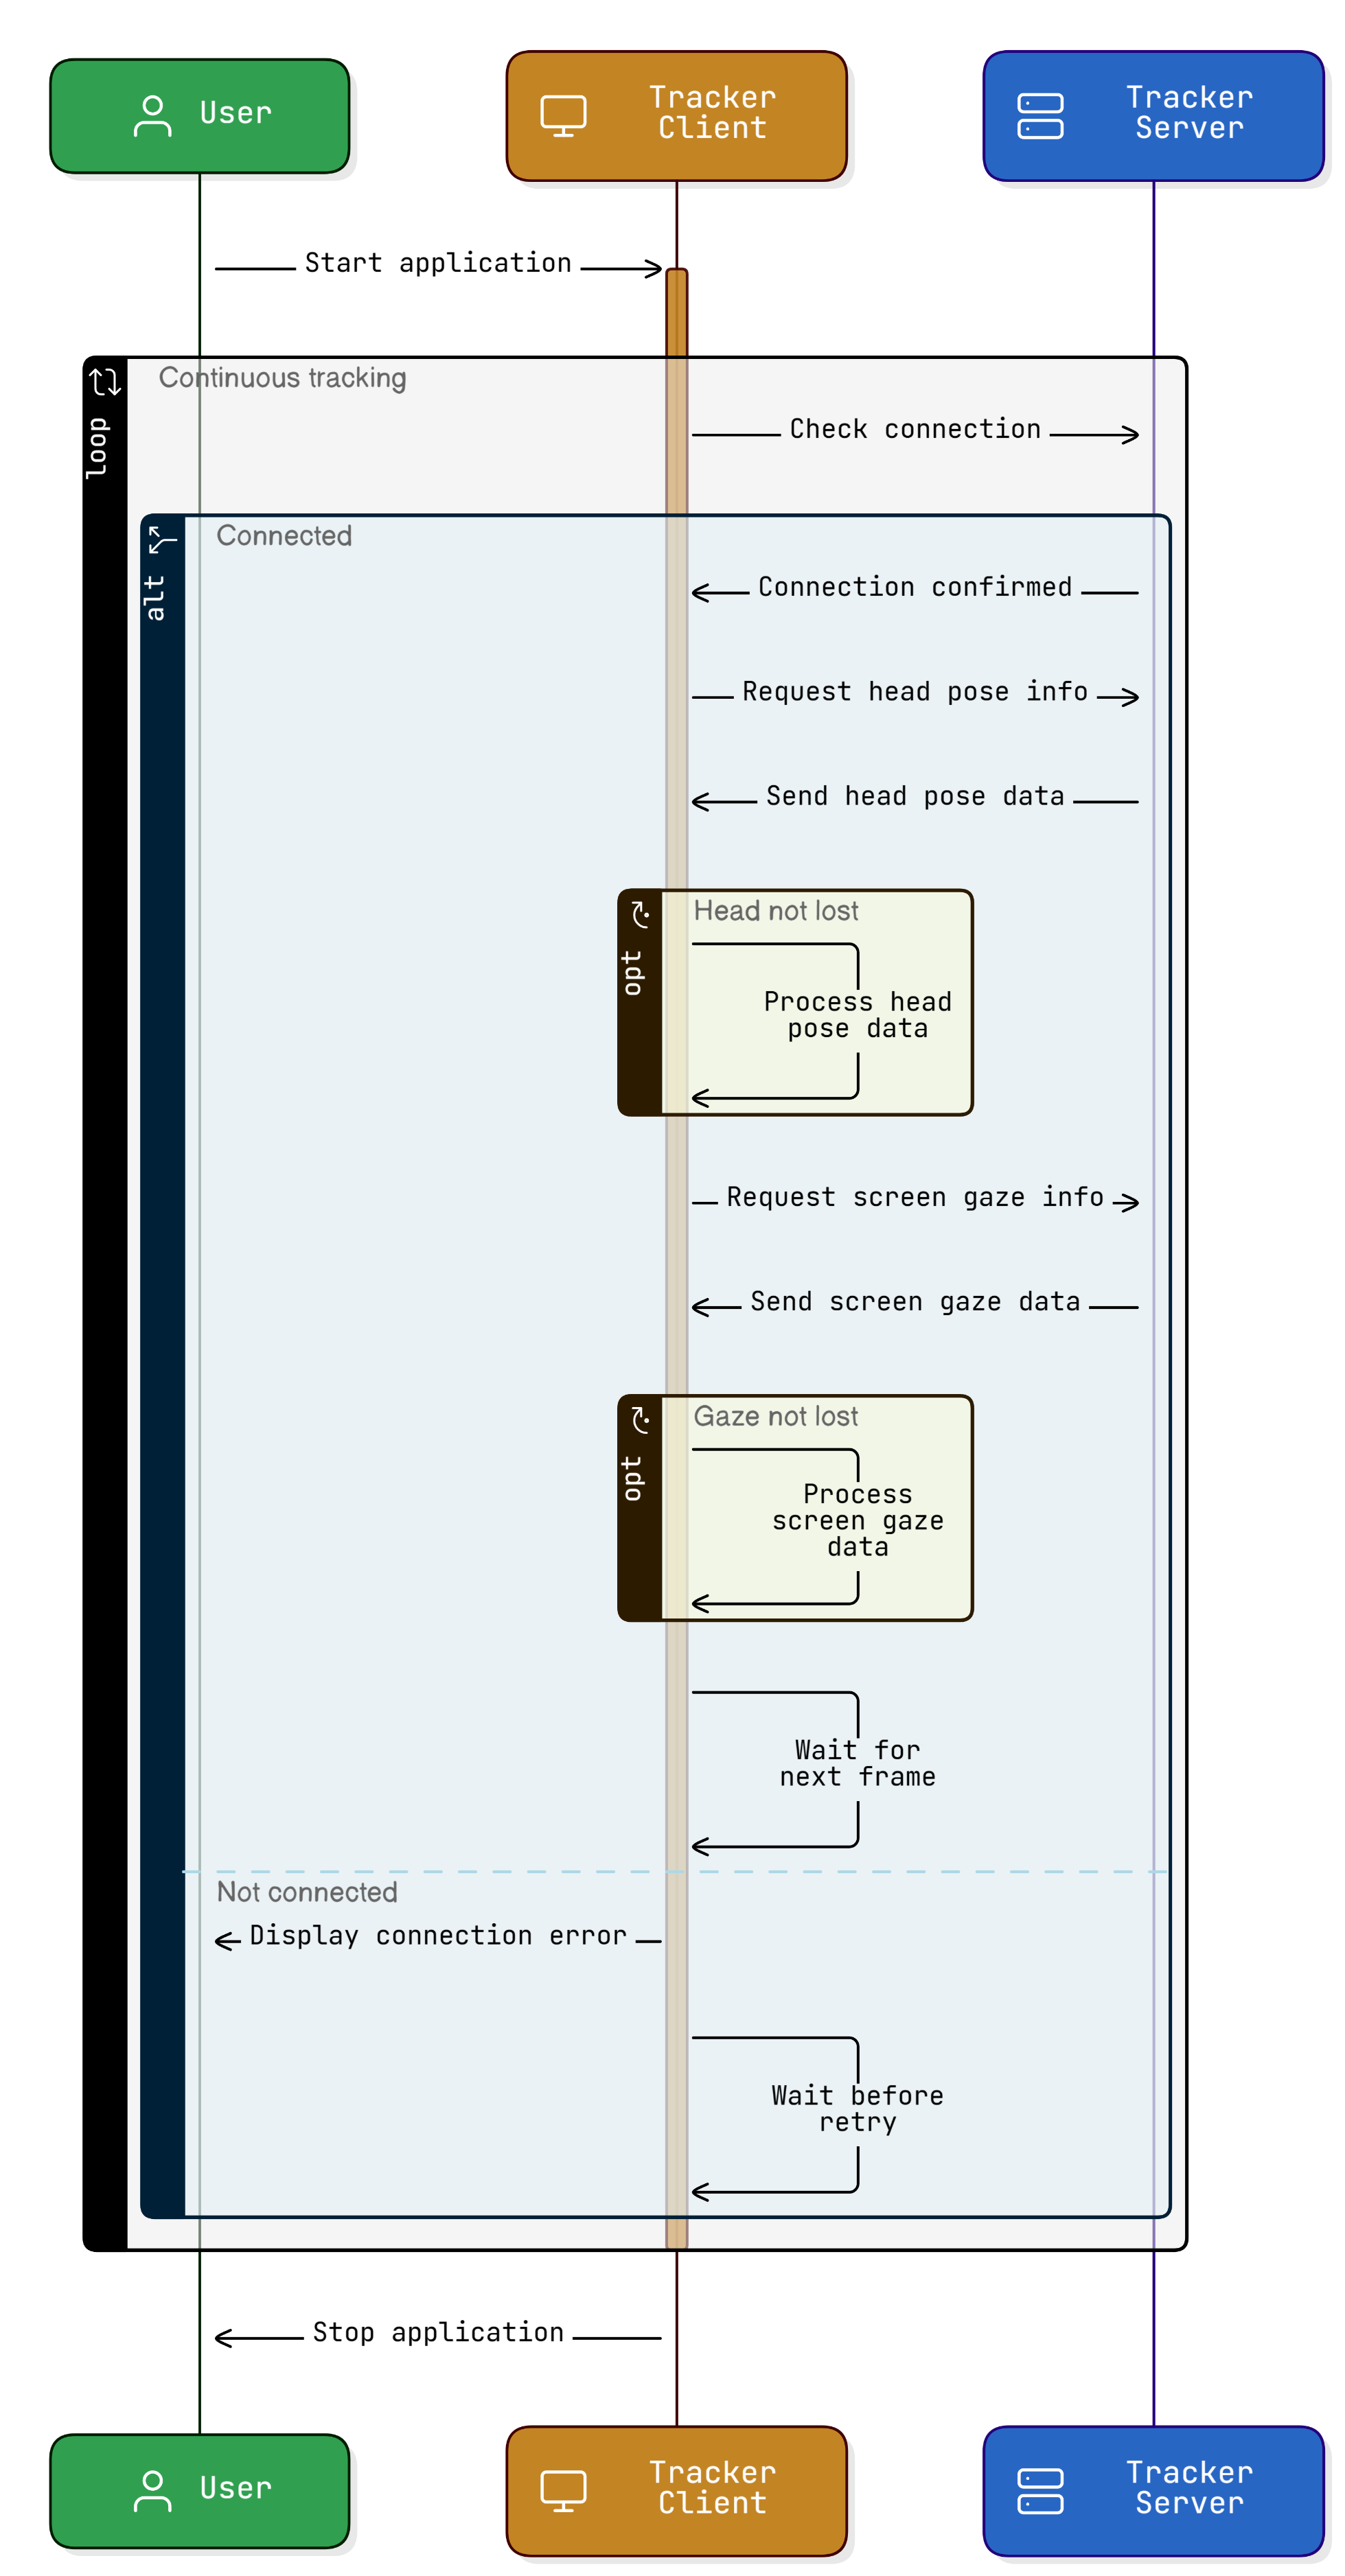
\includegraphics[scale=0.12]{code_structure_beam}
		\caption{Visuelle Darstellung des Codes zur Beam {\ac{SDK}}, Quelle: \cite{lit_code_beam_sdk}, \cite{lit_software_eraserio}} \label{fig:code_structure_beam}
	\end{center}
\end{figure}


Die Funktionsweise der {\ac{API}} ist vereinfacht in Abbildung \ref{fig:code_structure_beam} zu erkennen. Der Tracker Server ist die Bezeichnung für den Eye Tracker selbst. Der Client ist das selbst geschriebene Programm, welches die Trackerdaten über die {\ac{API}} entgegennimmt. Die beiden zentralen Informationen, welche vom Server an den Client übergeben werden sind die Daten zur Kopfposition (head pose data) und die Daten zur Blickposition (screen gaze data). Die Kopfposition gibt Auskunft über die Translation und Rotation des Kopfes der Testperson. Die Blickposition gibt Auskunft auf welchen Punkt auf dem Bildschirm die Testperson schaut. Diese beiden Systeme laufen unabhängig voneinander und dienen unterschiedlichen Einsatzzwecken. Das Kopftracking kann bspw. dazu dienen, die Kamera in einer Simulationswelt zu bewegen. Das könnte Sinn machen, wenn keine große Leinwand wie im Fahrsimulator vorhanden ist. Durch einen Blick nach links, könnte sich auch die Kamera im Fahrsimulator mit nach links bewegen. Für den Einsatzzweck im Fahrsimulator ist diese Funktion durch die große Leinwand allerdings nicht notwendig. Die Daten werden dennoch übermittelt, falls in Zukunft doch ein Anwendungsfall entstehen sollte. Die Gaze Daten stellen im Kontext dieser Arbeit die primär relevante Information dar. Diese geben eine Schätzung ab, auf welchen Punkt die Testperson auf der Leinwand schaut. Sofern eine Testperson vom Eye Tracker erkannt ist, werden in kontinuierlichen Abständen diese Daten vom Eye Tracker an den Client übermittelt. Zusätzlich dazu werden auch noch andere Daten wie bspw. die confidence übermittelt. Dabei handelt es sich um einen Wert, welcher mit jeder geschätzten Blickposition mit übermittelt wird. Dieser gibt an, wie sicher sich der Eye Tracker mit seiner Schätzung der aktuellen Blickposition ist. 

\section{Schnittstelle zu CARLA}

Im folgenden Abschnitt soll der Datenfluss zwischen CARLA und dem Eye Tracker sowie dem selbst geschriebenen Programm erläutert werden.
Der Eye Tracker und CARLA arbeiten größtenteils getrennt voneinander. Die visuelle Ausgabe des Eye Trackers erfolgt durch einen kleinen schwarzen Punkt, welcher die aktuell, geschätzte Blickposition auf der Leinwand anzeigt. Dieser schwarze Punkt befindet sich in einem selbst erstellten transparenten Fenster, welches über den Bildschirm gelegt wird. Der schwarze Punkt ist nicht Teil von CARLA oder dem Eye Tracker sondern wird durch das selbst geschriebene Programm erzeugt. Er basiert auf den x- und y-Koordinaten des Eye Trackers, welche durch eine zusätzliche Korrekturfunktion optimiert werden. Diese Korrektur wird in einem späteren Abschnitt genauer erläutert. Es gibt auch einen sogenannten Textmanager. Dieser ist auch selbst entwickelt und weder Teil von CARLA noch vom Beam Eye Tracker. In diesem werden für den Nutzer unter anderem die grobe Blickrichtung in Textform angezeigt. Zum Beispiel "schaut nach oben links". Der Text Manager wird wie in der Abbildung \ref{fig:eye_tracker_data} zu sehen ist mit Informationen des Eye Trackers und von CARLA gespeist.

Die einzige direkte Schnittstelle zwischen CARLA und den Daten des Eye Trackers ist die Übergabe der Eye Tracker Daten an die Auswertung des Instance Segmentation Sensors. Dieser Sensor wird in einem späteren Abschnitt genauer erläutert. Diese Schnittstelle funktioniert so, wie in Abbildung \ref{fig:eye_tracker_data} dargestellt. Der CARLA Server sendet die Sensordaten des Instance Segmentation Sensors an den CARLA Client. Der CARLA Client übergibt die Sensordaten an die Auswertung. Bei der Auswertung werden die Rohdaten des Eye Trackers, die zuvor durch eine Krümmungs-Korrektur angepasst wurden, dann mit den Sensordaten des Instance Segmentation Sensors verarbeitet. Durch die Kombination aus Eye Tracking Daten und den Daten des Sensors kann eine Aussage darüber getroffen werden, auf welches Objekt die Testperson innerhalb der CARLA Simulationswelt schaut. Diese Ausgabe wird dann im Text Manager in Form von Text auf dem Bildschirm dargestellt. Eine genaue Beschreibung der Funktionsweise der einzelnen Elemente folgt in späteren Abschnitten.
>>>>>>> fd0befd8e95e2bae230d21ece8a1862eada6b577


\begin{center}
	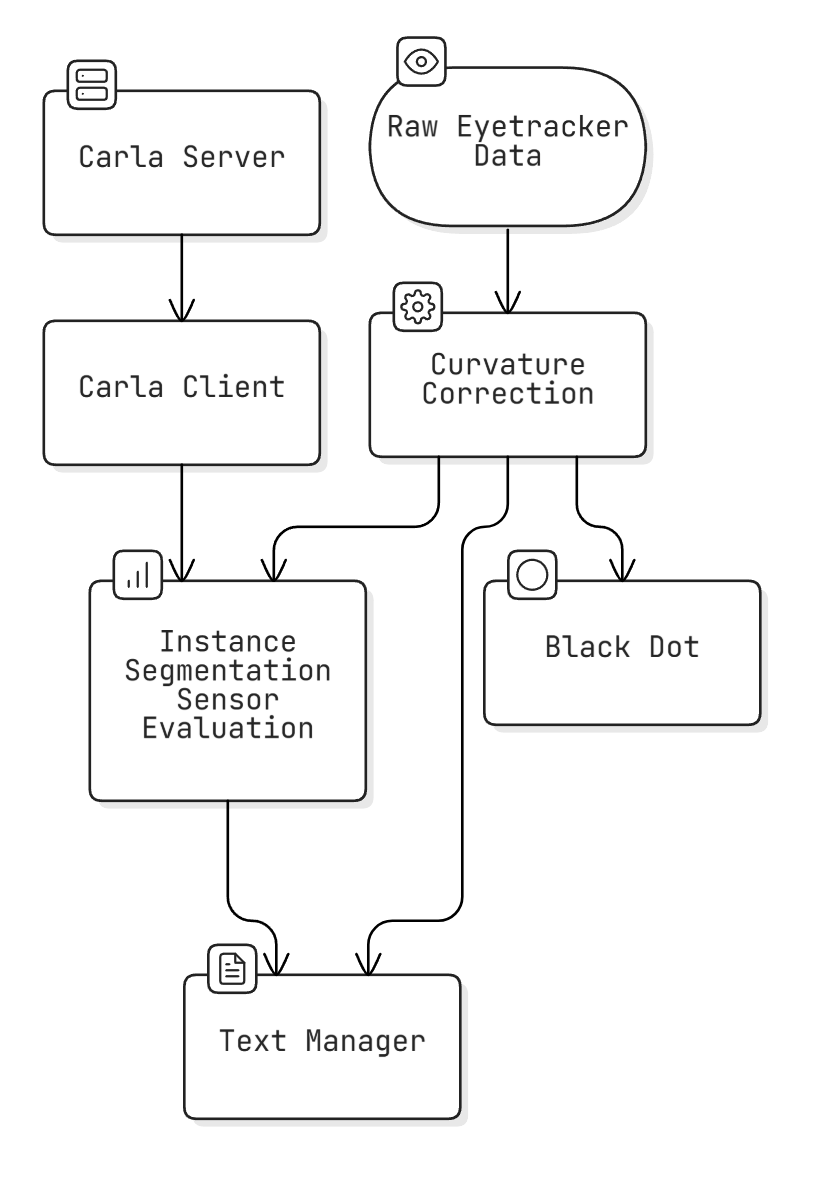
\includegraphics[scale=0.19]{eye_tracker_data}
	\captionof{figure}{Graphische Darstellung der Verarbeitung der Raw-Daten des Eye Trackers, Quelle: \cite{lit_website_carla_documentation}} \label{fig:eye_tracker_data}
\end{center}

	\input{mainmatter/CARLA Umgebung}
	\input{mainmatter/Korrektur gekrümmte Leinwand}
	\chapter{Auswertung}
\label{sec:auswertung}


\begin{figure}[h!]
	\begin{center}
		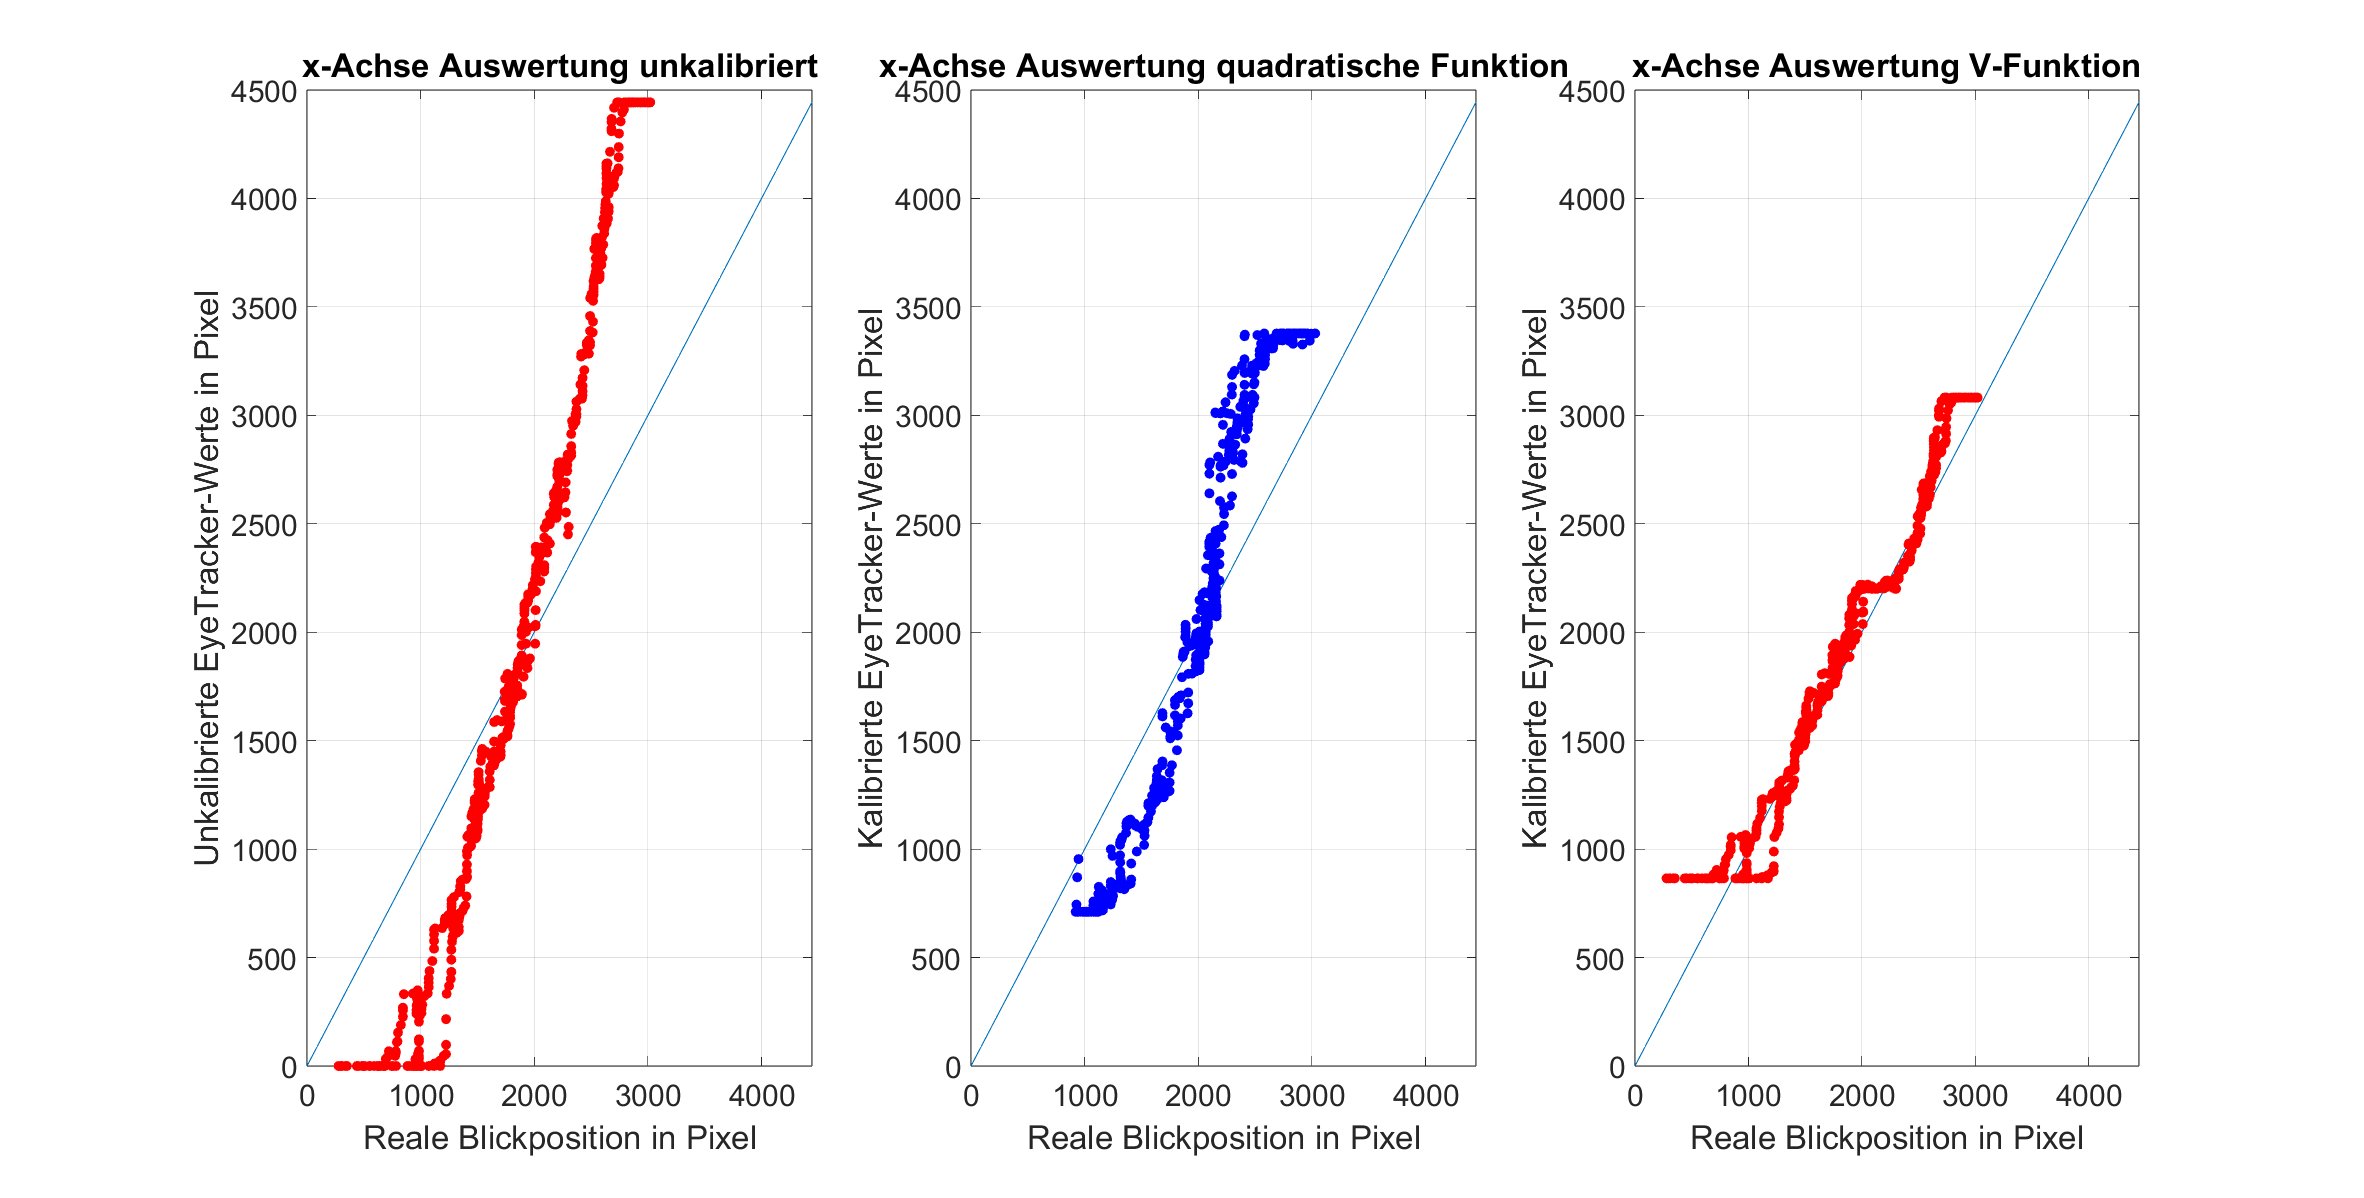
\includegraphics[scale=0.25]{second_correction_function_results_andold}
		\caption{Gegenüberstellung reale Blickposition und Eye Tracker-Werte: unkalibriert (links), kalibriert quadratische Funktion(mitte), kalibriert V-Funktion (rechts), Quelle: \cite{lit_software_matlab}} \label{fig:imag12}
	\end{center}
\end{figure}

In Abbildung \ref{fig:imag12} sind die Ergebnisse zu erkennen, welche mit der neuen v-förmigen Korrekturfunktion erzielt werden konnten. Es ist eine deutliche Verbesserung gegenüber der quadratischen Korrekturfunktion zu erkennen. Ein eingeschränkter Sichtbereich ist weiter vorhanden. Da ab einem gewissen Punkt allerdings sowieso keine verwertbaren Werte mehr geliefert werden ist das nicht problematisch. Der Eye Tracker korrigiert in der Nähe der Bildschirmmitte jetzt aggressiver und hat damit Erfolg. Auch in Randnähe wieder stärker korrigiert und somit der Fehler reduziert. Durch die unterschiedlichen Parameter für linke und rechte Bildschirmhälfte entsteht im Übergang von linker auf rechte Bildschirmhälfte und anders herum ein kleiner Sprung. Eine weitere Optimierung würde den Rahmen dieser Projektarbeit übersteigen. 

\begin{figure}[h!]
	\begin{center}
		
\includegraphics[scale=0.19]{second_correction_function_results_y}
		\caption{Gegenüberstellung reale Blickposition und Eye Tracker-Werte y-Achse kalibriert, Quelle: \cite{lit_software_matlab}} \label{fig:imag13}
	\end{center}
\end{figure}

In Abbildung \ref{fig:imag13} ist die Auswertung der y-Achse nach der Kalibrierung dargestellt. Auf den ersten Blick wirkt es so, als wären die Tracking Ergebnisse auf der y-Achse schlechter als auf der x-Achse. Das liegt allerdings zum Teil an der anderen Skalierung der y-Achse im Diagramm. Bei den horizontalen Pixelwerten in den Abbildungen weiter oben war die y-Achse von null bis 4444 skaliert. Die y-Achse für die vertikalen Pixelwerte ist allerdings nur von null bis 1080 skaliert. Eine Abweichungen von bspw. 300 Pixeln wirkt im Graphen für die vertikalen Pixel größer als im Graphen für horizontale Pixel. Ein anderer Grund ist, dass keinerlei Optimierung der vertikalen Pixel durch unseren Code vorgenommen wird. Für die Optimierung der horizontalen Pixel durch die Krümmung der Leinwand wurden große Aufwände betrieben. Durch eine Optimierung der vertikalen Pixel könnten evtl. noch weitere Verbesserungen erzielt werden.

	\chapter{Fazit}
\label{sec:fazit}

\section{Auswertung und Zusammenfassung}

Die im Rahmen der Projektarbeit definierten Zielsetzungen wurden erfüllt. Die Ergebnisse zeigen, dass es mit handelsüblicher Hardware (USB-Webcam) und sehr kostengünstiger Software möglich ist, bereits verwertbare Ergebnisse zu generieren. Ursprünglich war angedacht, eine Open-Source-Lösung als Fundament für den Eye Tracker zu verwenden. Nach ausgiebiger Marktrecherche konnte ein passendes Softwarefundament ausfindig gemacht werden. Der Beam Eye Tracker ist zwar nicht Open Source, aber die Daten, die er durch seine API bereitstellen kann, bieten genug Spielraum, um individuelle Lösungen damit bauen zu können. Eine Verschmelzung zwischen CARLA und dem Eye Tracker ließ sich ohne signifikante technische Herausforderungen realisieren. Die Daten aus dem Instance Segmentation Sensor können zusammen mit den Werten des Eye Trackers ausgewertet werden. Somit ist es möglich, nicht nur die geschätzten Koordinaten des Eye Trackers auf der Leinwand auszugeben, sondern auch das betrachtete Objekt innerhalb der CARLA Simulationsumgebung zu bestimmen.
Während der Implementierung des Eye Tracking Systems sind an manchen Stellen auch Probleme aufgetreten. Die Belichtung war vor allem während der Kalibrierung ein Problem. Durch verschiedene Ansätze und Experimente im Fahrsimulator konnten hier mit externer Belichtung gute Ergebnisse erzielt werden.
Eine weitere Herausforderung stellten die durch die gekrümmte Leinwand verfälschten Tracking Daten dar. Durch umfassende Analyse des Problems, einige mathematische Ansätze und Experimente im Fahrsimulator, konnte die daraus resultierende Abweichung signifikant reduziert werden. Die in Abbildung \ref{fig:imag12} dargestellten Ergebnisse zeigen, dass die korrigierten Daten eine deutlich verbesserte Genauigkeit aufweisen.
Die Tracking Daten sind allerdings nicht perfekt und lassen sich durch äußere Einflüsse wie schlechte Belichtung, Bedienungsfehler bei der Kalibrierung, Veränderung der Sitzposition nach der Kalibrierung oder zwei Personen gleichzeitig im Fahrsimulator negativ beeinflussen. Der Eye Tracker könnte allerdings zum aktuellen Entwicklungsstand bereits funktional im Fahrsimulator eingesetzt werden. Anhand der gemessenen Performance, deuten die Ergebnisse darauf hin, dass bereits mit dem aktuellen Entwicklungsstand verwertbare Blickdaten generiert werden können. Im Ausblick sollen weitere Schritte und mögliche Ideen präsentiert werden, mit welchen über diesen Low Budget Ansatz hinaus noch bessere Ergebnisse erzeugt werden könnten.


\section{Ausblick}

Aufbauend auf den Ergebnissen dieser Arbeit kann eine weitere Verbesserung des Testaufbaus erfolgen. Dazu zählen eine Ausbesserung der Lichtverhältnisse im Fahrsimulator, eine fest verbaute Kamera und gegebenenfalls eine Blende, sodass nur der Fahrer und nicht zusätzlich der Beifahrer von der Kamera erkannt wird. Ebenso kann die Eye Tracker Genauigkeit verbessert werden, indem die Korrektur für den gekrümmten Bildschirm durch einen potentiell noch besseren Optimierungsalgorithmus durchgeführt wird. Eine weitere Optimierungsmöglichkeit stellt die Anpassung der vertikalen Kalibrierung dar. Bspw. ließe sich dadurch ein statisches Offset korrigieren, wenn die Person während einer Fahrt in vertikale Richtung die Sitzposition verändert. Eine Integration von künstlicher Intelligenz zur Bestimmung der genauen Blickposition könnte ebenfalls die Genauigkeit verbessern. 
Abschließend bieten sich weiterführende Analysen an, wie eine zeitabhängige Auswertung von Blickpositionen in einem Zeitstrahl. 
Der Code des Eye Trackers ist dem Anhang beigefügt und kann somit weiterentwickelt werden.


\clearpage

	
	
	%%%%%%%%%%%%%%%%%%%%%%%%%%%%%%%%%%%%
	%	APPENDIX
	%%%%%%%%%%%%%%%%%%%%%%%%%%%%%%%%%%%%
	% Comment out or delete inputs you don't need. Add additional chapters if necessary
	\appendix
	\addtocontents{toc}{\protect\contentsline{chapter}{Appendix}{}{}}
	\chapter{Headline of Appendix A}
\label{sec:appendixA}

In principle, the appendix contains things that are too large or too extensive to be mentioned directly in the text:

\begin{itemize}
	\item Large tables
	\item Program code
	\item Large figures
	\item Measurement data	
	\item ...
\end{itemize}

Furthermore, the appendix can be used to give detailed explanations of aspects that are to long to cover them directly in background or state of the art chapters. The appendix can also be structured in chapters (\Cref{sec:appendixA}, \Cref{sec:appendixB}, ...)

	\chapter{Matlab Skripte \& Messwerte}
\label{sec:appendixB}

Der Code der Matlab Skripte zur Auswertung der Ergebnisse und zur Darstellung der Korrekturfunktionen sowie die Messergebnisse sind dem Projekt als digitaler Anhang beigelegt. Es wurde darauf verzichtet diesen hier einzufügen. 
Die Dateien befindet sich unter Anhänge -> Anhang B Matlab Skripte \& Messwerte.
	
	
	%%%%%%%%%%%%%%%%%%%%%%%%%%%%%%%%%%%%
	%	BACK MATTER
	%%%%%%%%%%%%%%%%%%%%%%%%%%%%%%%%%%%%
	% Comment out or delete inputs you don't need
	\backmatter
	\listoffigures
	\addcontentsline{toc}{chapter}{\listfigurename}
	\newpage
	\listoftables
	\addcontentsline{toc}{chapter}{\listtablename}
	\newpage
	\listofalgorithms
	\addcontentsline{toc}{chapter}{\listofalgorithmsname}
	\newpage
	\lstlistoflistings
	\addcontentsline{toc}{chapter}{\lstlistlistingname}
	\abbrevations{%%%%%%%%%%%%%%%%%%%%%%%%%%%%%%%%%%%%%%%%%%%%%%%%%%%%%%%%%%%%%%%%%%%%%%%%%%%%%%%%%%%%%%%%%%%%%%%%%%%%%%
%	COMMENTS
%%%%%%%%%%%%%%%%%%%%%%%%%%%%%%%%%%%%%%%%%%%%%%%%%%%%%%%%%%%%%%%%%%%%%%%%%%%%%%%%%%%%%%%%%%%%%%%%%%%%%%
% Headline is created automatically
% Add missing abbreviations
% Comment out abbreviations you don't need. Otherwise they will be displayed in this list even if you have not used them in text! 

\begin{acronym}
	\acro{IEEM}{Institut für energieeffiziente Mobilität}
	\acro{API}{Application Programming Interface}
	\acro{IR}{Infrarot}
	\acro{SDK}{Software Development Kit}
	\acro{USB}{Universal Serial Bus}
	\acro{HKA}{Hochschule Karlsruhe}
	\acro{RGB}{Rot, Grün, Blau}
	\acro{ID}{Identifikationsnummer}
\end{acronym}


}
	\symbollist{%%%%%%%%%%%%%%%%%%%%%%%%%%%%%%%%%%%%%%%%%%%%%%%%%%%%%%%%%%%%%%%%%%%%%%%%%%%%%%%%%%%%%%%%%%%%%%%%%%%%%%
%	COMMENTS
%%%%%%%%%%%%%%%%%%%%%%%%%%%%%%%%%%%%%%%%%%%%%%%%%%%%%%%%%%%%%%%%%%%%%%%%%%%%%%%%%%%%%%%%%%%%%%%%%%%%%%
% Headline is created automatically
% Adapt according to your needs


\label{sec:symbolsList}
\begin{table}[H]
	\centering
	\begin{tabularx}{\textwidth}{ll}
		$I$, $Item$ 			& Definition of a system model item 			 \\
		$Items$					& Set of all system model items 				 \\	
		$M_{Adjacent}$			& Adjacency matrix of the system model, which 	 \\
								& defines connected items						 \\
	\end{tabularx}
\end{table}}
	
	% Bibliography
	\printbibliography[heading=bibintoc]	
		
		
\end{document}

